\documentclass[12pt, twoside]{report}

\usepackage{shellesc}

\usepackage[a4paper,width=150mm,top=30mm,bottom=40mm,bindingoffset=6mm,headheight=10mm]{geometry}

\usepackage{fancyhdr}

%\usepackage{biblatex}
\usepackage[square,numbers]{natbib}
%\addbibresource{references.bib}
\bibliographystyle{abbrvnat}

\usepackage{graphicx}
\graphicspath{ {./images/} }

\usepackage{siunitx}

\usepackage{placeins}

\usepackage{csquotes}

\usepackage{enumitem}

%%% Tikz 
\usepackage{tikz}
\usepackage{pgfplots}\pgfplotsset{compat=1.18}
%\usepackage{pgfplotstable}
\usepackage{pgfmath}
\usetikzlibrary{arrows.meta,positioning,calc,intersections,external,shapes,angles,patterns,quotes}
\usepgfplotslibrary{units, groupplots, statistics, colormaps}

\usepgfplotslibrary{external}
\tikzexternalize
\tikzsetexternalprefix{figures/}
%\tikzset{external/force remake}
%\tikzset{external/remake next}

\newcommand{\inserttikzfig}[1]{
\tikzsetnextfilename{#1}%image name
\input{#1}}

\usepackage{amsmath} % for the equation* environment
\usepackage{amsfonts}
\usepackage{amssymb}

\usepackage{caption}
\usepackage{subcaption}

\usepackage{hyperref}

\usepackage{cleveref}

\crefname{figure}{figure}{figures}
\Crefname{figure}{Figure}{Figures}
\crefname{equation}{equation}{equations}
\Crefname{equation}{Equation}{Equations}

\newcommand{\mytitle}{Neuromorphic control of embodied central pattern generators}
\newcommand{\mysubtitle}{A neuromorphological approach to motion}
\newcommand{\myname}{Christian Fernandez Lorden}
\newcommand{\mychaptername}{Undefined}
\newcommand{\mychapterdesignation}{Chapter}
\newcommand{\mychapter}[1]{\chapter{#1}\renewcommand{\mychaptername}{\mychapterdesignation~\thechapter : #1}}

\pagestyle{fancy}
\fancyhead{}
\fancyhead[RO,LE]{\mytitle}
\fancyfoot{}
\fancyfoot[LE,RO]{\thepage}
\fancyfoot[LO,RE]{\mychaptername}
%\fancyfoot[CO,CE]{\myname}
\renewcommand{\headrulewidth}{0.4pt}
\renewcommand{\footrulewidth}{0.4pt}

\fancypagestyle{plain}{%
    \fancyhead{}
    \fancyfoot{}
    \fancyfoot[LE,RO]{\thepage}
    \fancyfoot[LO,RE]{\mychaptername}
    %\fancyfoot[CO,CE]{\myname}
    \renewcommand{\headrulewidth}{0pt}
    \renewcommand{\footrulewidth}{0.4pt}
}

\begin{document}
    \newgeometry{hmargin=2cm, vmargin=2cm}
\begin{titlepage}
    \centering
    
    \thispagestyle{empty}
    \vspace*{1cm}
        
    \Huge
    \textbf{\mytitle}
        
    \vspace{0.5cm}
    \LARGE
    \mysubtitle
        
    \vspace{1.5cm}
        
    {\bfseries \myname}
    
    \vfill
    
    
\includegraphics[width=\textwidth]{uliege_logo_rvb_pos.pdf}
    
    \vfill
    
    \Large
    \textbf{Supervisors :}\\
    Pr. Pierre Sacr\'e\\
    Pr. Guillaume Drion
    \LARGE
        
    \vfill
        
    Master's thesis completed in order to obtain the\\
    \textbf{Master of Science in Electrical engineering}
        
    \vspace{0.8cm}
        
        
    \Large
    University of Liege\\
    School of Engineering and Computer Science\\
    Academic Year 2022-2023
            
\end{titlepage}
\restoregeometry

    
    \thispagestyle{plain}
\begin{center}
    \Large
    \textbf{\mytitle}
        
    \vspace{0.4cm}
    \large
    \mysubtitle
        
    \vspace{0.4cm}
    \textbf{\myname}
       
    \vspace{0.9cm}
    \textbf{Abstract}
\end{center}
The control of robotic locomotion poses important challenges. In particular, we are still very far from achieving in robotic locomotion control with the same degree of robustness and adaptability to unexpected environmental perturbations exhibited by moving biological systems.

In my master thesis research, I use biological neuron models to create artificial CPG to control a simple mechanical system in a robust and efficient manner. Akin to \citet{CPGRobot}, my inspiration is the known electrophysiology, sensory response, and modulation of biological CPGs \citet{crayfish,stickInsect,MARDER}.

My research started by exploring how a single neuron is able to robustly generate a high-amplitude periodic motion in a simple resonant mechanical system (a pendulum) without fine tuning of the neuron parameters and with weak sensory feedback and actuation. I found that only if the motor neuron exhibits a robust type of bursting \citet{burstingSlowFeedback,Franci2} it is able to robustly and rapidly adapt its excitable behavior to the unknown mechanical system's properties (damping, resonant frequency, mass, etc.).

I am now exploring how to use a pair of bursting neurons in a push-pull configuration to simultaneously achieve robust amplitude and oscillation frequency control and how to create network of bursting neuron to achieve robust and adaptable spatio-temporal coordination of coupled mechanical systems, akin to multi-legged 
locomotion.

The hope is that a good and robust control over simple mechanical systems is the first step toward efficient adaptive walking.


    \renewcommand{\mychaptername}{Abstract}

    %\chapter*{Dedication}
    %To mum and dad

    %\chapter*{Declaration}
    %I declare that..

    %\chapter*{Acknowledgements}
    %I want to thank...
    
    
    \tableofcontents
    \renewcommand{\mychaptername}{Contents}
    

    \mychapter{Introduction}
    In robotics, the control of locomotion still presents significant difficulties.
On one hand, we are currently distant from attaining the level of robustness and adaptability to unforeseen changes in the environment that is demonstrated by living organisms. 
On the other hand, the mobile nature of most robots forces them to resort to batteries or other embedded energy sources to power themselves. 
However, an embedded energy source often means that energy becomes a valuable resource for the robot. 
This limits the power that can be allocated to onboard computing, leading to a trade-off between power allocated to computing and autonomy and increasing the difficulty of creating robust controllers. 

To solve this energy and robustness problem, new approaches are emerging. 
One of them is neuromorphic engineering, which aims to extract the useful properties of biological neuronal systems to create highly efficient artificial neuronal controllers or processing units.

While not directly related to robotics, a relatively classic and old but still striking example is the game of Go between Lee Sedol and AlphaGo \citep{alphago1,alphago2,alphago3}. 
This match marked the first time a top-tier Go player was beaten by an AI. While this appears to contradict the first sentences of this paragraph, an aspect that should not be overlooked is the power consumed by both player. 
\citet{alphagoenergy} cite that AlphaGo needed around \qty{1}{\mega\watt} of power to play Go, while Lee Sedol brain only sipped around \qty{20}{\watt}, while also performing other tasks such as processing visual information. 
This shows that the current machine learning approach achieves impressive performance but, even with current improvements \citep{alphagolessenergy}, fails to even approach the power efficiency and versatility of neuronal structures.
In comparison, the human brain is an extremely energy-efficient processor. 
It is capable of simultaneously processing audio, visual, and other sensory feedback while making decisions based on incomplete knowledge. 
Neuromorphic engineering tries to reproduce the efficiency that was seen in the brain or other biological systems.

For motion, multiple researches \citep{crayfish,stickInsect,MARDER} show that simple neuronal systems called central pattern generators (CPGs) are the basis of motion in nature. 
\citet{crayfish} shows that this system is the basis of the movement of the crayfish while \citet{stickInsect} proves a similar thing for the stick insect.
It is thought that these basic systems exhibit very important properties that are the reason for their success.

\section{Problem Statement}

This thesis investigates the control of a simple resonant mechanical system (a pendulum).
Traditionally, the control of such a system is achieved through a PID using trajectory tracking or other continuous controllers. 
%These controllers often work in a very restrained pendulum size space and require additional controllers to achieve gaits between multiple pendulums.

%In accordance with the limitations laid earlier, 
This thesis aims to create and analyze an artificial neuronal controller capable of generating sustained oscillations of a simple pendulum.
The generated oscillation must be regular, and the amplitude of this motion should be dynamically controlled using an external parameter.
To achieve this goal, this thesis explores the concepts of excitability and CPGs to create a more robust controller.

%I aim to create a neuromorphic controller capable of generating a sustained oscillation that tunes its oscillations to reach an amplitude based on the value of an external input.

To be clearer, the controller should fulfill the following properties.
\begin{itemize}
    \item Be an end-to-end neuromorphic controller
    \item Act by generating torque at the attachment point.
    \item Use only the angular position and velocity as observed variables
    \item Maintain stable symmetric oscillations
    \item Regulate oscillations to achieve the desired amplitude 
    \item Be resilient to inaccuracies in the controller parameters
    \item Respect the natural frequency of the system
\end{itemize}

\section{Related literature}

For this thesis, two fields of study are relevant because the thesis sits at their intersection. These are the fields of neuromorphic control and pendulum control.

Strangely enough, very little literature exists on the control of a simple pendulum. The best match is the work of \citet{Pendulum3} which is based on \citet{Pendulum3comp} and develops a controller for regulating the energy of a pendulum attached to a cart. This is similar to regulating the amplitude because a given amount of energy can be linked to a certain amplitude. 

Others are more distant from the classical pendulum. \citet{Pendulum2} explore to control of a pendulum with propellers attached on its side using an adaptive Kalman filtering PID. While \citet{Pendulum1} are interested in controlling the swing of a leg system using a H2 full state feedback with a PID controller.

Conversely, extensive literature exists on neuromorphic control. Like \citet{neuromorph1} who designed a biomimetic controller for biped motion control. Or \citet{cpgmotorpattern} which proposed a new CPG structure for motion control. Many articles could be cited, but suffice it to say that the field is gaining traction. No article was found that directly solved the problem of pendulum swing, but the closest subject would probably be bipedal locomotion on which many people have done research \citep{related2,related5,neuromorph1,related4}.

From this research, it seems that the problem presented in this thesis has not yet been considered. However, perhaps it was a sub-problem of some other research that was not found.

\section{Structure and remarks}

This thesis is divided into multiple chapters with distinguishing themes.
\begin{description}
 \item[Chapter 2: Neurons and CPGs] This chapter serves as an introduction to the field of neuromorphic engineering. This section explains and defines the terms specific to this domain that are used throughout the thesis.
 \item[Chapter 3: Modeling and analysis of neuronal circuits] In this chapter, the models of neurons and synapses that are used to create the controller are defined. It also explores the behavior of the neuron model as a function of its parameters.
 \item[Chapter 4: A neuromorphic sensorimotor loop for pendulum swing] In this chapter, the main problem of the thesis is addressed. Two models of controllers are defined and analyzed. The goal is to determine which subspace of parameters leads to a strong connection between the controller and the mechanical system.
 \item[Chapter 5: Neuromodulation for adaptive amplitude control] This chapter expands the model found in the previous chapter to include a system capable of modifying the controller parameters to achieve a desired amplitude.
 \item[Chapter 6: Simple interconnection of controller-pendulum systems] The last chapter briefly explores the idea of generating specific spatiotemporal patterns between pendulums by interconnecting their controllers.
\end{description}
Note that throughout the thesis, multiple parameters are assigned units. These units distinguish the role that the parameters play in the models. They do not represent actual physical quantities. 

Also, the thesis rely on multiple metrics to make decision or compare sets of parameters. \Cref{apx:algos} contains the explanation of the metrics as well as the algorithms used to compute them.

\iffalse
To reuse an somewhat old but striking example, in 2016 AlphaGO bested one of the best human go player. Yet, AlphaGO consumed around \qty{1}{\mega\watt} to accomplish this feat while the brain of Lee Sedol, the human player, only consumed around \qty{20}{\watt}. And, in addition to playing the game, Lee's brain also processed all its sensory inputs, controlled its arm to make the moves on the board and continued regulating the equilibrium of its body. Better yet, after the game, he was able to go home and perform activities that are fundamentally different from playing go.

This energy gap between machine and human is explained by the fundamental difference in their computational architecture. The traditional architecture uses synchronized computing steps with memory separated from the computing. Conversely, in a neuronal net, the computing is done completely asynchronously and the memory of the systems is integrated in the computing since it is represented by the dynamical nature of the neurons.
\fi

    
    \mychapter{Neurons and CPGs}
    % Principle of models 
    % CPG and feedback => embodied
    % Rhytms , excitablility
    % Connection of CPG and motor rythms
    \label{sec:neuro_expl}

In this thesis the concepts specific to neuromorphic engineering will be used extensively. 
Before diving into the design and results of the proposed controllers, a clear understanding of these and other related concepts must be reached. 
Otherwise, comprehension of the choices or design decisions made will be difficult.

\section{Excitability}

The first step in the comprehension of neuronal system is the concept of excitability. In the words of \citet{excDef}, \enquote{Excitability is the property of a system to exhibit all-or-none response to pulse inputs}. 
In other words, the system exhibit nearly no response from pulses until the pulse amplitude crosses a certain threshold after which the system responds completely. 

In \cref{fig:excitability}, an example of an excitable behavior is displayed. 
As can be seen, a very small difference in the pulse amplitude resulted in a very different neuronal behavior. 
The lower pulse resulted in the output faithfully following the input while the output of the higher one exhibited a very different behavior with oscillation and  peaks far above the input. 
This specific behavior is known as bursting and will be discussed later.

\begin{figure}[htb]
    \centering
    \inserttikzfig{plots/excitability.tikz}
    \caption{Example of an excitable behavior. Generated using neuron model of \cref{sec:model}.}
    \label{fig:excitability}
\end{figure}

This kind of behavior is often seen in neuronal systems.
The all-or-none response is important to transform continuous input into discrete events. 
This discretization makes a system more resilient to noise and capable of reacting only when necessary.

This kind of response is desired in our controller since the effective control of the oscillation of a pendulum requires a very all-or-nothing control input. 
Indeed the moment of actuation is very important when controlling a pendulum and actuating at a bad time can lead to very poor results. 
Still, in  the words of \citet{excDef}, \enquote{\textins{Excitability} is instrumental in converting sensory signals into motor actions}.

To create an excitable system a localized positive feedback loop is necessary. 
Indeed, the switch between two different responses after the crossing of a threshold requires the activation of a positive feedback near the threshold. 
This feedback pushes the output of the system to generate the excitable event.

\section{Conductance-based neuron models}

Excitability being defined, neuronal models can be understood more clearly. Indeed, neurons are a prime example of an excitable system.

Basically, neurons are cells that are able to receive input from the external world, send messages to one another and send motor commands to muscles. 
Since a neuron can be relatively big, it is evident that its behavior may be different at different part of the cell. 
But, a common way to observe a neuron is to measure and model its activity in only one location.

As shown by \citet{neuronIons}, the state of a neurons at its axon membrane can be described by the flow of ionic currents. 
The magnitude of those current is determined by the potential across the interior and the exterior of the cell which opens or closed channels at a speed that is dependent on the channel type.
In turn these currents flowing into or out of the cell influence the potential across the interior and the exterior of the cell. 

This model is illustrated on \cref{fig:conductance_neuron}, where ionic currents are flowing through channels in the neuron membrane. Those channels activate and deactivate based on the membrane potential.

\begin{figure}[htb]
    \centering
    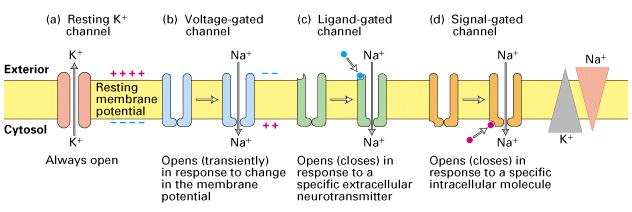
\includegraphics[width=.9\textwidth]{channels.png}
    \caption{Simplified diagram of a biological neuron membrane. (Diagram taken from \citet{channelDiagram})}
    \label{fig:conductance_neuron}
\end{figure}

\begin{figure}[htb]
    \centering
    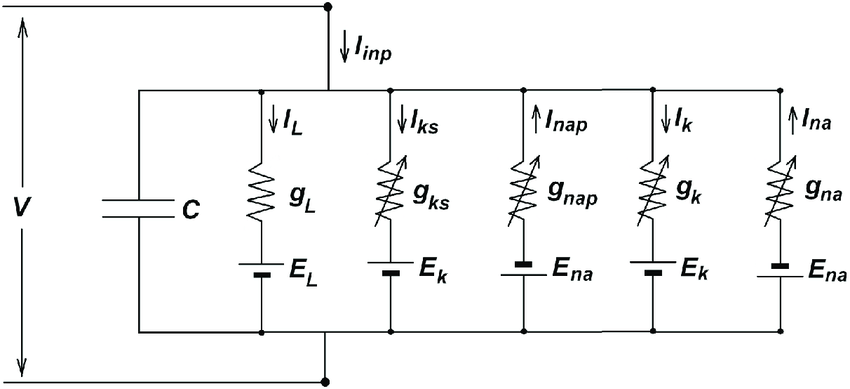
\includegraphics[width=.9\textwidth]{conductanceNet.png}
    \caption{Simplified circuit of the neuron model. (Circuit taken from \citet{electricDiagram})}
    \label{fig:conductance_neuron_circuit}
\end{figure}

This language of currents and potential seems to designate classical circuit theory as a useful tool to model a neuron behavior.
\citet{conductanceModel} were the first to formulate a model of the neuronal behavior using a parallel network of dynamic conductances. 
Those conductances change based on the membrane voltage of the neuron at different rates mimicking the opening and closing of the channels. 
A good representation of this model is seen in \cref{fig:conductance_neuron_circuit}. 
On this diagram, it can be seen that some ionic current discharge the capacity that represent the membrane while other charge it. 
Those charging current effectively act as positive feedback loops. 
As seen in the previous section, those are necessary for the excitable behavior of a neuron.

Using circuit theory, this model can be written more formally using ordinary differential equation. 
\Crefrange{eq:hodgkinstart}{eq:hodgkinend} are a very general representation of this model.
In this representation the $i$ subscript denotes the different ionic currents that can be found in \cref{fig:conductance_neuron_circuit}.

\begin{align}
    C\frac{\partial V}{\partial t} =& I_\text{inp} - g_L\left(V-E_L\right) - \sum_i I_i\label{eq:hodgkinstart}\\
    I_i\left(t, V\right) =& g_i\left(t, V\right)\left(V - E_i\right)\\
    g_i\left(t, V\right) =& \bar{g_i}m_i\left(t, V\right)^{p_i} h_i\left(t, V\right)^{q_i}\\
    \frac{\partial m_i\left(t, V\right)}{\partial t} =& \frac{m_{i\infty}\left(V\right) - m_i\left(t, V\right)}{\tau_{mi}\left(V\right)}\\
    \frac{\partial h_i\left(t, V\right)}{\partial t} =& \frac{h_{i\infty}\left(V\right) - h_i\left(t, V\right)}{\tau_{hi}\left(V\right)}\label{eq:hodgkinend}
\end{align}

The $m_\infty$, $h_\infty$, $\tau_m$ and $\tau_h$ terms follow saturation functions.
The saturation of the $\infty$ terms show that the ionic current feedbacks are localized in a certain range of membrane voltage.
This was expected since excitable behavior requires a localized positive feedback.


This model is very general and, when parameters are chosen properly, it is able to generate a whole range of neuronal behaviors seen in biological neurons. 
In this thesis, only spiking and bursting, the two most common behaviors will be used. Those two behaviors can be seen in \cref{fig:behaviours}. 
A spike is a sudden, short and steep increase in the neuron voltage followed by a sharp decrease and return to a resting voltage. 
A burst is the apparition of a packet of spikes.

Classically both behaviors can be tonic of phasic.
A tonic response means that it is sustained, this is what is observed in \cref{fig:behaviours} where the spike and burst repeat.
A phasic response means that it is transient, the behavior is only caused by a change in the input like in \cref{fig:excitability} and will not continue after the initial response.
Often, for a set of parameters, as the input current increases a neuron will first have a phasic response before starting to become tonic.
% Tonic or not tonic bursting and spiking

\begin{figure}[htb]
    \centering
    \inserttikzfig{plots/neuron_behaviour.tikz}
    \caption{Example of spiking and bursting behaviors. Generated using neuron model of \cref{sec:model}.}
    \label{fig:behaviours}
\end{figure}

\section{Neuronal Behavior Metrics}

As seen before neural behaviors exhibit unusual patterns. 
To be able to compare different bursting or spiking specific metrics must be defined.
Here, only the metrics to evaluate the tonic spiking and the tonic bursting will be discussed.

\Cref{fig:burst_metrics} represents values that can be directly inferred from the trance of a tonic bursting neuron. Those values can be defined as
\begin{description}
    \item[Burst length] The average time of a burst event.
    \item[Rest length] The average time of inactivity between two burst events.
    \item[Burst period] The average time between the starts of two burst events.
    \item[Spike period] Inside a burst, the average time between the start of two spike events.
    \item[Number of spikes] The average number of spikes inside a burst event.
\end{description}

\begin{figure}[htb]
    \centering
    \inserttikzfig{diagrams/burst_metrics.tikz}
    \caption{Illustration of the different metrics used to describe bursting. Generated using neuron model of \cref{sec:model}.}
    \label{fig:burst_metrics}
\end{figure}

Aside from the number of spikes, those raw metrics metrics are not suited to this thesis. 
Instead, the following set of metrics derived from the aforementioned values is used.
\begin{description}
    \item[Inter-burst frequency] $\frac{1}{\text{Burst period}}$, the frequency at which burst events occur.
    \item[Intra-burst frequency] $\frac{1}{\text{Spike period}}$, frequency at which spikes occur inside a burst event.
    \item[Duty cycle] $\frac{\text{Burst length}}{\text{Burst period}}$, the portion of time of a period where the neuron is inside a burst event.
    \item[Number of spikes] The average number of spike inside a burst event.
\end{description}
Even though the inter-burst frequency and the intra-burst frequency are just opposites of direct metrics, the realm of frequencies is often better suited to compare with other things.


The tonic spiking does not require so much metrics. 
The only direct metric is measuring the \textbf{Spike period}.
It is enough to compute the \textbf{Spiking frequency} which is the most useful metric to describe a spiking behavior. 
For the same reason as the bursting transforming in frequencies is better for comparison.


% Types

\section{Central Pattern Generators and Rhythms}

To develop the controller, the concept of central pattern generators (CPGs) is very useful since they are linked closely to rhythmic movement. 
And, the oscillation of a pendulum is a naturally rhythmic movement.

From \citet{cpgDef}, \enquote{A central pattern generator (CPG) is an assembly of neurons that possesses the ability to produce a rhythmic activity pattern without \textdel{phasic} sensory feedback information}.

From this, it id clear that CPGs require multiple neurons to work.

Also, it is widely admitted that central pattern generators are frequently found in biological motion systems. 
\citet{cpgMotion, cpgMotion2} highlight that CPGs are abundant in the control of animals motion.
The natural periodic oscillations of CPGs makes them easier to pair with systems that are already periodic

To keep it simple, the connections between neurons inside a CPG result in the activity of one neuron generating currents in the other neuron. 
Those connections can have two types, inhibitory and excitatory. 
An inhibitory connection results in negative current being injected while an excitatory connection creates a positive current.

The most simple and well studied CPG is the half-center oscillator \citep{halfcenter}. 
This specific circuit is composed of two neurons that inhibit each other. 
The system along with simulation can be seen in \ref{fig:halfcenter}.
The currents flow from one neuron to the other only if the injecting neuron is activated.

\begin{figure}[htb]
    \centering
    \inserttikzfig{diagrams/halfcenter.tikz}
    \caption{Example of an half center oscillator. Traces were generated using neuron model of \cref{sec:model}.}
    \label{fig:halfcenter}
\end{figure}

The generation of rhythmic patterns is clear when looking at the traces of the activation of the different neurons. 
Indeed, the activation of neuron 1 and neuron 2 always follow each other.
This temporal shift can be expressed in term of phase by saying that one neuron as a phase of $\frac{1}{2}$ of a period compared to the other.
But, it will no appear in the game.
% Cite marder or other of different CPGs, show graphs of rythms

\section{Embodied Intelligence and CPGs} 

From \citet{embodiedDef} \enquote{Embodied intelligence is the computational approach to the design and understanding of intelligent behavior in embodied and situated agents through the consideration of the strict coupling between the agent and its environment (situatedness), mediated by the constraints of the agent’s own body, perceptual and motor system, and brain (embodiment).}.

This concept is describing the goal of this thesis.
Indeed , the model that is developed later is a prime example of embodied intelligence. 
The controller will process direct sensory input to generate coherent control signals for the motor. Using neuromodulation the strength of the push will be changed according to a desired amplitude.

More broadly, the concept of embodied intelligence is closely related to CPGs. Indeed, CPGs are circuits that are rhythmic without sensory feedback, but using sensory feedback to tune the frequency of the CPG to the external is thought to be inner working of most biological motion controller (citation needed).
This coupling is precisely a low-level embodied intelligence. 

To Simplify embodied intelligence, it can be seen as the coupling of sensing computing and actuating. 
The agent in embodied learning has its sensors, its computing and its actuation in the same body. 


% Define embodied Intelligence and its relationship with CPGs 

    
    \mychapter{Modeling and analysis of neuronal circuits.}
    \label{sec:model}

%Now that the essential behaviors linked to neurons are defined the analysis of the neuronal model can begin.
Building upon the concepts defined previously, this chapter aims to show and study the different possible behaviors that the neuronal model can exhibit.
In more detail, a quick explanation of the model is provided, followed by a general analysis of the active regions of the model. Then, a more detailed analysis of specific parameter values is conducted for some bursting and some spiking.
The discussion will also include the definition of synapses and their use to create a half-center oscillator.

\section{ODEs of the Neuronal Model}

The backbone of the model used is based on a model developed by Pr. A. Franci.
A diagram representing this model can be seen in \cref{fig:neuron_mod}. 
The diagram shows that the  model is composed of four different internal variables.
The membrane potential $V$, the fast voltage $v_f$, the slow voltage $v_s$ and the ultra-slow voltage $v_u$.
The system also has a single input $I_\text{app}$ the applied current.
This block diagram can be easily translated into ODEs because it is composed only of functions and first-order low-pass filters.
\Crefrange{eq:neur_start}{eq:neur_end} are a more formal description of the neuron model.

\begin{figure}[!hb]
    \centering
    \inserttikzfig{diagrams/neuron_model.tikz}
    \caption{Diagram of the Neuron Model. The output of the neuron is $V$ and the input is $I_\text{app}$.}
    \label{fig:neuron_mod}
\end{figure}

\begin{align}
    \tau_o\frac{\partial V}{\partial t} &= V_0 + I_\text{app} - i_{f-} - i_{s+} - i_{s-} - i_{u+} - V\label{eq:neur_start}\\
    i_{f-} &= g_{f-}\left(\tanh\left(v_f-d_{f-}\right) - \tanh\left(V_0-d_{f-}\right)\right)\\ 
    i_{s+} &= g_{s+}\left(\tanh\left(v_s-d_{s+}\right) - \tanh\left(V_0-d_{s+}\right)\right)\\ 
    i_{s-} &= g_{s-}\left(\tanh\left(v_s-d_{s-}\right) - \tanh\left(V_0-d_{s-}\right)\right)\\ 
    i_{u+} &= g_{u+}\left(\tanh\left(v_u-d_{u+}\right) - \tanh\left(V_0-d_{u+}\right)\right)\\ 
    \tau_f\frac{\partial v_f}{\partial t} &= V - v_f\\
    \tau_s\frac{\partial v_s}{\partial t} &= V - v_s\\
    \tau_u\frac{\partial v_u}{\partial t} &= V - v_u\label{eq:neur_end}   
\end{align}
with $g_{f-},\, g_{s-} < 0$, $g_{s+},\, g_{u+} > 0$ and $d_{f-},\, d_{s+},\, d_{s-},\, d_{u+} \in \mathbb{R}$.

Here $i_{f-}$ is the fast positive feedback to the neuron, $i_{s+}$ and $i_{s-}$ are the slow negative and positive feedback and $i_{u+}$ is the ultra-slow negative feedback. $+$ represents negative feedback and $-$ represents positive feedback because, in electrical notation, the current is oriented to discharge the neuron. Therefore, an increase in the current tends to decrease the membrane voltage, whereas a decrease in the current tends to increase the membrane voltage.

$i_{s+}$ and $i_{s-}$ could be written as a single current because they are on the same timescale $v_S$.
However, since they play a different role in the behavior of the neuron and to maintain the symmetry between the currents, they are written separately.

This model displays local positive feedback both with $i_{f-}$ and $i_{s-}$.
As seen in the previous chapter, this positive feedback is necessary for excitable behaviors.
More precisely, this model follows the findings of \citet{burstingSlowFeedback}.
They stated that tunable and robust neuronal behavior must include slow positive feedback.
Slow in this context means in a timescale between the fast positive feedback that creates the spike and the ultra-slow feedback that slowly brings the neuron back to a resting voltage.
In this model, the $i_{s-}$ currents fill this role.
Designing a system with this slow feedback should make its bursting more resilient to changes in other parameters.

%This model is clearly a simplified version of a conductance based model, with the conductance changing at different time scale though the multiple time scale of the voltages and the saturation coming from the $\tanh$ function.
This model is a simplification of a conductance-based model with four currents on three fixed timescales and variable conductances replaced by a low-pass filter followed by explicit voltage-to-current relationships.
The model being written in the language of currents and voltages is reminiscent of the origin of this model.

For this thesis, some parameters of the model will remain fixed at the following values. Exploring these parameters does not lead to interesting results that are not reachable without tuning them. 
{

\large\centering
\begin{tabular}{lr|lr}
    $V_0$    & \qty{-0.85}{\volt} & $\tau_{o}$ & \qty{0.0004}{\second}\\
    $d_{f-}$ & \qty{0.0}{\volt}   & $\tau_{f}$ & \qty{0.001}{\second}\\
    $d_{s+}$ & \qty{0.5}{\volt}   & $\tau_{s}$ & \qty{0.04}{\second}\\
    $d_{s-}$ & \qty{-0.5}{\volt}  & $\tau_{u}$ & \qty{0.8}{\second}\\
    $d_{u+}$ & \qty{-0.5}{\volt}  & &
\end{tabular}

}

To ensure the stability of the models, it is always a good idea to apply some noise to simulate real-world conditions.
In the case of the neuron, the best way to add noise easily is to add it to the input current.
In this way, noise affects the entire neuron. This is also a good way to represent real use because in an integrated chip, most of the noise should come from the outside world. 

To better understand the inner workings of the neuron, \cref{fig:neuron_inside} shows a representation of the currents and voltages of the model during a simulation. 

The low-pass filter effect is very clear when looking at the different voltages.
$v_f$ is nearly indistinguishable from $V$ due to the very high cutoff frequency of the filter.
$v_s$, on the other hand, follows the general pattern of the bursting but has a cutoff frequency low enough to filter the spikes inside the burst.
$v_u$ filters the bursting and follows a smooth sawtooth pattern, rising during the burst and falling down during the inactivity between bursts.

The saturation of the current is very visible when looking at the flat regions of some currents, especially $i_{s+}$, which is nearly a flat line between the bursts.
This indicates the inactivation of the slow negative feedback because changes in voltages do not result in changes in $i_{s+}$.
Furthermore, the "launching" effect of the slow positive feedback is visible.
$i_{s-}$, is the first current to activate with a slow slope before the burst and seems to start the burst by activating $i_{f-}$.
Then, the increase in voltage seems to launch $i_{f-}$ which starts the first spike of the burst. 
This indicates a $i_{f-}$, $i_{s+}$ pair that is more closely linked with the spikes inside the burst and a $i_{s-}$, $i_{u+}$ pair that is more associated with the burst itself.

\begin{figure}[!htb]
    \centering
    \inserttikzfig{plots/neuron_inside.tikz}
    \caption{Currents and voltages inside the neuron model. Currents share the color of their generating voltages.}
    \label{fig:neuron_inside}
\end{figure}

\section{Behavior of neuron in function of its parameters}

Before designing a controller, the behavior of the neuron under different parameters must be studied to determine the best parameters for the controller.
For this analysis, only an exploration of the parameters $g_{s-}$, $g_{u-}$ and $I_\text{app}$ is done since they are the parameters most relevant to bursting.
$g_{f-}$ and $g_{s+}$ are fixed to $g_{f-} = \qty{-2}{\siemens}$ and $g_{f-} = \qty{6}{\siemens}$ since those parameters gave good bursting behavior.

Firstly, \cref{fig:neuron_activation} displays an overview of the different regions where the neuron is active.
More precisely, it distinguishes between different activation types. Here 3 different activation types are considered.
Spiking and bursting, which were defined in the previous chapter, and plateau, which is short for plateau bursting.
Plateau bursting is a degenerate form of bursting that sees the apparition of a plateau voltage between the first spike and the rest of the spikes of the burst. 
In extreme cases, plateau bursting stops containing any spike other than the first spike, and the behavior becomes analogous to periodic pulses.

For this thesis purpose, the bursting region is the most interesting because it allows tunability by playing with intra- and inter-burst characteristics.

In this configuration, the bursting region seems to advance with an increase in the applied current until $I_\text{app}=\qty{0}{\ampere}$ then in recedes, seemingly pushed by the spiking region.
The border between normal bursting and plateau behavior seems to follow a line that does not really depend on $I_\text{app}$.
This border indicates that the plateau behavior is mostly dependent on the value of $g_{s-}$ and nearly independent of the value of $g_{u+}$.
The shape of this boundary is probably controlled by $g_{f-}$ and/or $g_{s+}$.
The parameters at the center of the chart are capable of sustaining bursting for various applied currents.
Indeed, a neuron with $g_{s-} \approx \qty{-4}{\siemens}$ and $g_{u+} \approx \qty{5}{\siemens}$ seems to be in a very stable bursting zone for the controller. It can sustain bursting from $I_\text{app} = \qty{-1.8}{\ampere}$ to $I_\text{app} = \qty{2}{\ampere}$ and seems far enough from plateau bursting to never show unwanted behaviors.

\begin{figure}[!htbp]
    \centering
    \begin{subfigure}[t]{\textwidth}
        \centering
        \caption{Map of neuron activation types with $g_{f-} =  \qty{-2}{\siemens}$ and $g_{s+} =  \qty{6}{\siemens}$.}
        \inserttikzfig{plots/neuron_type.tikz}
    \end{subfigure}
    
    \begin{subfigure}[b]{\textwidth}
        \centering
        \caption{Traces of the three different neuron activation types. Computed using $I_\text{app} = \qty{-1}{\ampere}$, $g_{u+} = \qty{6}{\siemens}$ and $g_{s-}  \in \left\{\num{-6},\,\num{-4},\,\num{-2}\right\}\unit{\siemens}$.}
        \inserttikzfig{plots/neuron_type_ex.tikz}
    \end{subfigure}
    \caption{Different types of neuron activation. The plateau region corresponds to the bursting region, where a voltage plateau exists between the first spike and the rest of the spikes.}
    \label{fig:neuron_activation}
\end{figure}

Now that the good region has been highlighted, a closer look at the inter-burst frequency will be useful to categorize bursting.
Indeed, it is better to have neurons attuned to the frequency of the pendulum to obtain good results.
However, let us keep in mind that for large swings, the frequency of the pendulum depends on the amplitude of the swing; therefore, a perfect match for changing amplitudes will probably not be found.
In \cref{fig:neuron_burts}, it can be seen that the inter-burst frequency is mostly determined by the value of the conductances and not the applied current.
Changing the applied current mostly only changes the zone where bursting occurs.
The applied current still has an effect on the frequency, higher currents leads to a slightly higher frequency.
However, changing the values $g_{s-}$ and $g_{u+}$ has a far greater effect on the inter-burst frequency.
Note that the inter-burst frequency is also computed on the plateau behavior.
The continuity between both behaviors shows that the plateau behavior is actually just degenerate bursting.

\begin{figure}[!htb]
    \centering
    \inserttikzfig{plots/neuron_burst.tikz}
    \caption{Map of neuron bursting frequency with $g_{f-} = \qty{-2}{\siemens}$ and $g_{s+} =  \qty{6}{\siemens}$.}
    \label{fig:neuron_burts}
\end{figure}

However, by performing a finer analysis on $I_\text{app}$, another zone of bursting can be discovered.
In \cref{fig:neuron_burts_fragile}, this zone is highlighted.
This bursting occurs in a zone with nearly no slow positive feedback.
Yet, \citet{burstingSlowFeedback} indicated that the slow positive feedback is integral to a reliable bursting.
The lack of robustness of this bursting can already be inferred from the extent to which the zone of bursting shifts when subject to a small change in the input current.
In addition, the boundary of bursting seems more diffuse and the inter-burst frequency inside the zone does not seem to not follow a continuous pattern.
All these signs point toward this zone being an unreliable bursting behavior.
Still, a more detailed analysis to show the fragility of this bursting is necessary to eliminate it completely as a possibility.

\begin{figure}[!htb]
    \centering
    \inserttikzfig{plots/neuron_burst_close.tikz}
    \caption{Map of neuron bursting frequency with $g_{f-} = \qty{-2}{\siemens}$ and $g_{s+} =  \qty{6}{\siemens}$. Zoom on specific $I_\text{app}$ with apparitions of another bursting region.}
    \label{fig:neuron_burts_fragile}
\end{figure}

\Cref{fig:neuron_burts_comp} shows a comparison of the simulations of the stable bursting found earlier and the "fragile" bursting discovered here with and without noise.
This reveals that "fragile" bursting is totally destabilized by the addition of a small noise.
The regular two-spike pattern that appears without noise ceases to exist, and the number of spikes per burst and the inter-burst frequency seem to be very random.
The spikes probably correlate with the noise inside the neuron.
On the other hand, the "stable" burst seems unaffected by the noise.
The only visual indicator of the added noise is the shape of the voltage during the resting period, where small oscillations caused by the noise can be observed.
The number of spikes and the inter-burst frequency of stable bursting remain unchanged by noise.
This proves that the region of "stable" bursting is a far better burst than the region of "fragile" bursting since the first is resistant to noise and the latter is not.

This behavior is probably due to "stable" bursts being launched by $i_{s-}$ and the "fragile" burst being launched by $i_{f-}$ since $i_{s-}$ is nearly zero.
The filtering of noise is far better for $v_s$ than for $v_f$ because of the lower cut-off frequency of $v_s$.
Thus, the variable $v_f$ that launch the "fragile" burst is greatly affected by the noise, leading to the noise being able to launch a burst.
On the other hand, what launches the "stable" bursting nearly unaffected by the noise, leading to almost no change in the behavior of the neuron.
% Maybe make a plot but time is short

\begin{figure}[!htb]
    \centering
    \inserttikzfig{plots/burst_stable_fragile.tikz}
    \caption{Comparison of both times of bursting at $I_\text{app}=\qty{0.2}{\ampere}$. The stable model used $g_{s-}=\qty{-4}{\siemens}$ and $g_{u+}=\qty{5}{\siemens}$ and fragile model used $g_{s-}=\qty{-0.2}{\siemens}$ and $g_{u+}=\qty{4}{\siemens}$. The applied noise had a spectral power density of  $n_{I_\text{app}} = \qty{3e-7}{\volt\squared\per\hertz}$.}
    \label{fig:neuron_burts_comp}
\end{figure}
%% Plot montecarlo analysis (necessary ?)

\section{Bursting neuron characteristics}

In this section the changes in bursting behavior through the modification of certain parameters are studied.
Some analyses or graphs will only be performed with one set of parameters for bursting. Nonetheless, the conclusions drawn will hold for most of the normal bursting region and especially for the bursting region of interest in this thesis. 

\subsection{Spike number modulation with $g_{s-}$}\label{sec:spike_mod}
% Add a graph of the number of spikes per burst

A simple way to change the amount of power transmitted by a burst is to change the number of spikes in the burst.
Indeed, if $g_{f-}$ and $g_{s+}$ are fixed, the spike uptime will remain nearly the same regardless of the values of $g_{s-}$ and $g_{u+}$.
This leads to the number of spikes being the most important metric for characterizing the power transmitted by the spikes.
Indeed, the integral of the positive value of the membrane voltage can be seen as very strongly correlated with the number of spikes in the burst.

Both $g_{s-}$ and $g_{u+}$ could be used to modulate the number of spikes. 

But, \cref{fig:neuron_burts} shows that the value of $g_{u+}$ is more important to guarantee the existence of bursting at a specific $I_\text{app}$.
Indeed, the range of $g_{s-}$ where bursting exists is almost constant at $\left[-4;\;-2\right]\unit{\siemens}$ for all $I_\text{app}$.
On the other hand, the range of where bursting exists for $g_{u+}$ varies from $\left[6;\;9\right]\unit{\siemens}$ to $\left[1;\;9\right]\unit{\siemens}$ as $I_\text{app}$ goes from \qty{-2}{\ampere} to \qty{0}{\ampere}.
Thus, $g_{s-}$ will be used as the parameter to modulate the number of spikes because it is less likely to annihilate bursting.

The effect of this modulation can be seen in \cref{fig:neuron_burst_spikes} where the value of $g_{s-}$ is varied while counting the number of spikes.
The graph shows a clear link between the number of spikes in the burst and the value of $g_{s-}$ parameter.
The number of spikes decreased "linearly" as the amplitude of the feedback decreased.
Since the number of spikes must obviously be an integer, "linearly" means that the width of a region with a certain number of spikes is nearly constant.
Thus, the shape can be regarded as rounding the value of a linear function.
This trend holds until the number of spikes hits one and the neuron starts spiking instead of bursting.

\begin{figure}[!htb]
    \centering
    \inserttikzfig{plots/spike_burst_curve.tikz}
    \caption{Curve of the number of spikes as a function of the $g_{s-}$ parameter. With $I_\text{app} = \qty{-1}{\ampere}$, $g_{f-} = \qty{-2}{\siemens}$, $g_{s+} = \qty{6}{\siemens}$ and $g_{u+} = \qty{5}{\siemens}$.}
    \label{fig:neuron_burst_spikes}
\end{figure}

The explanation of why the number of spikes is strongly linked to the power transmitted was slightly ad hoc.
To confirm that this metric correlates well with the amount of power transmitted by the burst, a comparison with other metrics is necessary.
The metrics proposed for comparison with the number of spikes are the duty cycle of the burst and the mean positive value of the bursting.
The mean positive value is a value defined as
\begin{align}
    \text{mean positive value} = \frac{1}{T}\int_{t_0}^{t_0+T} \text{max}\left(0, V(t)\right) \mathop{\mathrm{d}t} 
\end{align}
The mean positive value is interesting because, in this thesis, when the membrane voltage is negative, the neuron is always considered inactive.
Of these two metrics, the mean positive value is obviously the most reliable; however, it is also interesting to see how well the duty cycle correlates with this value.

\Cref{fig:neuron_burst_power} displays the plot of these two metrics as a function of $g_{s-}$ values like in \cref{fig:neuron_burst_spikes}.
Analyzing this figure reveals that the number of spikes is indeed correlated with the power transmitted because the mean positive value is nearly constant with the number of spikes.

\begin{figure}[!htb]
    \centering
    \inserttikzfig{plots/power_burst_curve.tikz}
    \caption{Curve of the burst power as a function of the $g_{s-}$ parameter. With $I_\text{app} = \qty{-1}{\ampere}$, $g_{f-} = \qty{-2}{\siemens}$, $g_{s+} = \qty{6}{\siemens}$ and $g_{u+} = \qty{5}{\siemens}$.}
    \label{fig:neuron_burst_power}
\end{figure}

In addition, these figures show that the duty cycle is a poorer indicator of power because it can have the same value at two very different values of $g_{s-}$.
Moreover, at two $g_{s-}$ where the duty cycles are equal, the number of spikes and the mean positive value are very different, indicating poor performance of the metric.
In fact, the duty cycle follows a sawtooth pattern in which it grows with $g_{s-}$ but then has a large discontinuity when the number of spikes changes.
It appears that increasing $g_{s-}$ (thus reducing its effect) decreases the intra-burst frequency until a spike drops and the frequency returns to a higher level.
The observation of the intra-burst frequency is linked to the fact that a lower frequency leads to a larger burst, which means a larger duty cycle.

To confirm this explanation, \cref{fig:neuron_burst_intra} plots the intra-burst frequency as a function of $g_{s-}$ and shows that this is indeed the case.
The intra-burst frequency has a strange relationship with $g_{s-}$ as increasing $g_{s-}$ can locally increase the intra-burst frequency but globally decrease it.

\begin{figure}[!htb]
    \centering
    \inserttikzfig{plots/intra_burst_curve.tikz}
    \caption{Curve of the intra-burst frequency as a function of the $g_{s-}$ parameter. With $I_\text{app} = \qty{-1}{\ampere}$, $g_{f-} = \qty{-2}{\siemens}$, $g_{s+} = \qty{6}{\siemens}$ and $g_{u+} = \qty{5}{\siemens}$.}
    \label{fig:neuron_burst_intra}
\end{figure}

This entire analysis was performed because changing the power transmitted by the burst is integral to the control of the pendulum.
This power is linked to the torque applied to the pendulum, and controlling this torque is necessary to control the oscillation amplitude.
Having a good understanding of the modulation of $g_{s-}$ is thus crucial to the creation of a robust controller.

\subsection{Inter-burst frequency modulation with $g_{p+}$}

To obtain a reliable control, it is necessary for the natural frequency of the neuron to be close to that of the pendulum.
Otherwise a good coupling between both systems will not be possible.

Since $g_{s-}$, will be modulated to change the power of a burst, $g_{u+}$ must be used for the modulation of the inter-burst frequency.
$g_{s-}$ cannot be used because it will not be fixed in the final controller, rendering any analysis worthless.

\Cref{fig:neuron_burst_freq} shows the influence of the parameter and the applied current on the inter-burst frequency.
Interestingly, the limit between bursting and silence seems to follow a linear relationship between $I_\text{app}$ and $g_{u+}$ in this model.
This is probably an artifact of the specific values of other parameters and is not a general behavior of this neuronal model.
The inter-burst frequency seems to be mostly dependent on $g_{u+}$ when far away from the bursting boundary.
When approaching the boundary, the frequency quickly decreases compared with that further inside the boundary.
Therefore, in that region, the applied current starts to have a larger impact on the frequency.
A higher $g_{u+}$ leads to a higher oscillation frequency but also to an earlier activation of bursting.
A link can be made with \cref{fig:neuron_activation} where the higher the value of $g_{u+}$ the longer the neuron stays in the bursting region.

\begin{figure}[!htb]
    \centering
    \inserttikzfig{plots/freq_burst_map.tikz}
    \caption{Map of the inter-burst frequency as a function of the $g_{u+}$ parameter. With $g_{f-} = \qty{-2}{\siemens}$, $g_{s+} = \qty{6}{\siemens}$ and $g_{s-} = \qty{-4}{\siemens}$.}
    \label{fig:neuron_burst_freq}
\end{figure}

This analysis does not have the same goal as the previous one because no neuromodulation of $g_{u+}$ is done in this thesis.
Rather, it allows us to better understand later why some parameter values will lead to better control of the pendulum.
It was also used to slightly guide the design of the controller by restricting the parameter space for the bursting neurons

\section{Tonic spiking type-I neuron characteristics}
% Good parameter map for -2 4 parameters

For sensory feedback, a tonic type-I spiking neuron will be useful because it will be able to transform continuous signals into discrete events.
A neuron of that type can sustain spiking because it is tonic and has a spiking frequency that is closely correlated with the input because it is type-I.
These are the definitions of both terms.
This type of neuron is useful for sensory inputs because it is event based but keeps a trace of the strength of the input through the spiking frequency.

The following neuron will deviate from the standard values of $g_{f-}$ and $g_{s+}$ defined previously.
These values were chosen for bursting, and here spiking is of interest.
A detailed exploration of the parameter space was not performed either because only a single set of parameters is needed.
Indeed, modulation is not necessary for the sensory neurons in this thesis.

Now, in \cref{fig:neuron_spiking}, the firing frequency of the neuron is plotted in function of the input current. 
This figure clearly shows that for low values of applied current the spiking frequency is very strongly related with the input current. 
For higher currents the frequency saturates and even decreases before the spiking disappears.
But, this behavior happens at very high input current and the neuron frequency is very close to a linear function of the input for $I_\text{app} \in \left[0;\;1\right]\unit{\ampere}$.
In normal use the neuron will never be subject to current high enough to make it exit the region of linearity.
Thus, the poor performances at high input current are not problematic.

\begin{figure}[!htb]
    \centering
    \inserttikzfig{plots/fi_curve.tikz}
    \caption{F-I curve of a type I neuron. With $g_{f-}=\qty{-2}{\siemens}$, $g_{s+}=\qty{4}{\siemens}$, $g_{s-}=\qty{-1}{\siemens}$ and $g_{u+}=\qty{1}{\siemens}$. The curve starts and ends at the beginning and end of spiking.}
    \label{fig:neuron_spiking}
\end{figure}

The correlation of the applied current with the spiking frequency is necessary to obtain a good representation of the input at the output of the neuron. 
Indeed, the neuron is supposed to convert the amplitude of the input into a frequency.

\section{ODEs of the synaptic connections}

After studying a single neuron, networks of neurons must be considered to generate more complex spatiotemporal patterns.
Biologically, a classical way in which two neurons are connected is through a synapse.
A synapse is a connection between two neurons that allows the membrane voltage of the presynaptic neuron to generate a current in the postsynaptic neuron.
\Cref{fig:synapse_mod} show the diagram of the synapse model that will be used in this thesis. 

Similar to the neuron model, the synapse model comprises a low-pass filter followed by a nonlinear voltage-to-current function.
The synapse takes the voltage of a neuron as input and produces a current that can be fed as input to another neuron.
It is similar to the feedback system inside the neuron model with the difference that the current generated is not drained from the membrane potential of the presynaptic neuron but fed to the postsynaptic neuron.
The difference thus lies in the receiver and the sign of the current.

\begin{figure}[!htb]
    \centering
    \inserttikzfig{diagrams/synapse_model.tikz}
    \caption{Diagram of the synapses model. The output of the synapse is $I_\text{out}$ and the input is $V_\text{in}$.}
    \label{fig:synapse_mod}
\end{figure}


More formally, this model can be written as a simple ODE.
\begin{align}
    \tau_\text{syn}\frac{\partial v_\text{syn}}{\partial t} &= V - v_\text{syn}\label{eq:syn_start}\\
    i_\text{out} &= g_\text{syn}\sigma\left(4\left(v_\text{syn} - d_\text{syn}\right)\right)\label{eq:syn_end}   
    %\frac{\tanh\left(2\left(V-d_\text{syn}\right)\right)+1}{2}
\end{align}
with $g_\text{syn}\,, d_\text{syn} \in \mathbb{R}$ and $\sigma\left(\right)$ the sigmoid function.

The factor 4 inside the sigmoid increases its slope to obtain a faster transition and makes the slope at $d_\text{syn}$ equal to $1$, similar to the $\tanh$ function inside the neuron.

When the input neuron is inactive, its voltage is negative; thus, the sigmoid function is nearly zero and no current is sent to the post-synaptic neuron.
When the neuron is active, the sigmoid is non-zero and may even saturate to 1 and a current is sent to the post-synaptic neuron.
The sign of $g_\text{syn}$ will  decide if the synapse is excitatory or inhibitory.
A negative conductance creates an inhibitory connection that drains current, and a positive conductance creates an excitatory connection that injects current.

For this thesis, some parameters of the synapses will be fixed because changing them is not necessary to achieve the various objectives.
{

\large\centering
\begin{tabular}{lr|lr}
    $d_\text{syn}$    & \qty{0.0}{\volt} & $\tau_\text{syn}$ & \qty{0.04}{\second}
\end{tabular}

}

\section{Half center oscillator analysis}

Formed by the interconnection of two neurons linked by two inhibitory synapses, the half-center oscillator (HCO) is a central component of the controller. 
A representation of an HCO was already presented in \cref{sec:neuro_expl} by \cref{fig:halfcenter}.
A more detailed representation using specific parameters can be seen in \cref{fig:cpg_time}.

\begin{figure}[!htb] % Necessary
    \centering
    \inserttikzfig{plots/cpg_output_plot.tikz}
    \caption{Plot of the neuronal output of a CPG. With $g_{f-}=\qty{-2}{\siemens}$, $g_{s+}=\qty{6}{\siemens}$ ,$g_{s-}=\qty{-4}{\siemens}$, $g_{u+} = \qty{3.7}{\siemens}$, $I_\text{app} = \qty{-1}{\ampere}$, $g_\text{syn} = \qty{-1}{\siemens}$.}
    \label{fig:cpg_time}
\end{figure}

Being the assembly of two bursting neurons, the most interesting thing to study and control in the HCO is its frequency.
This frequency can be evaluated by the inter-burst frequency of one of its neurons because this frequency is the frequency of one cycle, and an HCO is defined as the alternating activation of two neurons.
\Cref{fig:cpg_act} depicts this frequency as a function of $I_\text{app}$ and $g_{u+}$ for a selection of $g_\text{syn}$.
These maps are similar to \cref{fig:neuron_burst_freq} where the inter-burst frequency was studied for a single neuron over the same parameters.
Low values of $g_\text{syn}$ lead to behaviors very similar to those of uncoupled neurons, whereas higher values lead to lower frequencies.
Similarity is expected since $g_\text{syn} = 0$ results in two uncoupled neurons.
The strength of the connection has a large impact on the behavior of the system.
The frequency is probably lowered by the larger values because a higher current lowers the membrane voltage of the neuron and the neurons take more time to correct this lower voltage.

\begin{figure}[!htb]
    \centering
    \inserttikzfig{plots/cpg_activation.tikz}
    \caption{Activation of the cpg network as a function of ultraslow negative feedback and applied current. With $g_{f-}=\qty{-2}{\siemens}$, $g_{s+}=\qty{6}{\siemens}$, $g_{s-}=\qty{-4}{\siemens}$.}
    \label{fig:cpg_act}
\end{figure}

A nice thing to note is that by comparing the HCO with the uncoupled case, it appears that the zone of bursting becomes larger as the strength of the connection increases.
This leads to the apparition of zones where bursting emerges from the network of neurons as the neurons alone are silent.
To further demonstrate this, \cref{fig:cpg_only_act} represents only the zones where bursting is caused by the network and not the intrinsic properties of the neurons.
The higher the connection between the neurons is the larger the zone of bursting is.

\begin{figure}[!htb]
    \centering
    \inserttikzfig{plots/cpg_only_activation.tikz}
    \caption{Activation of the cpg network as a function of ultraslow negative feedback and applied current. Only the region where the bursting arises from the network is shown. With $g_{f-}=\qty{-2}{\siemens}$, $g_{s+}=\qty{6}{\siemens}$, $g_{s-}=\qty{-4}{\siemens}$.}
    \label{fig:cpg_only_act}
\end{figure}

%In short the higher the interconnection the more the network is able to burst but it does so with a lower inter-burst frequency. 


    \mychapter{A neuromorphic sensorimotor loop for pendulum swing}
    \label{sec:pendulum}

The previous chapter explored the different behaviors exhibited by the neuron model.
This chapter will focus on the control of a cylindrical pendulum with a neuromorphic controller built using neurons.
The primary goal is to find and extract a control scheme that is intrinsically linked with the mechanical system.
To reach this goal the different useful behaviors of the neuron model will be paired with multiple feedback models. 
The models will be evaluated on their performances and their robustness.

\section{The mechanical system}

Before diving into controller design, understanding the mechanical system is important. 
\Cref{fig:pendulum} shows a graphical representation of the system. 
This diagram shows that there is only a single control input to this system, the applied torque $\tau$. 
The system also gives two meaningful state output, the angle $\theta$ with the vertical and the angular velocity $\dot{\theta}$. 
Finally the dynamics of the pendulum are influenced by 5 parameters, the radius $r$ of the cylinder, the height $h$ of the cylinder, the density $\rho$ of the cylinder, the damping coefficient $B_f$ which generates the friction torque $\tau_f$ at the rotation point and the gravity $\mathbf{g}$. 
\begin{figure}[!htb]
    \centering
    \inserttikzfig{diagrams/pendulum_system.tikz}
    \caption{Diagram of the pendulum system. The parameters of the pendulum are in blue, the output that are fed to the controller are in red and the actuation of the controller is in green.}
    \label{fig:pendulum}
\end{figure}

On the figure, the gray gray arrow shows and defines the down direction which is the reference of the angle $\theta$. 
It can be used to separate the rotation plane in two halves. 
The half with negative $\sin\left(\theta\right)$ and the half with positive $\sin\left(\theta\right)$.

For this controller the parameters of the pendulum will be kept constant. 
%Keeping the parameters in a certain close range is obviously necessary.
%A controller capable of stabilizing the oscillation of a \qty{1}{\milli\meter} pendulum will struggle and fail when applied on a \qty{1}{\meter} long pendulum. Keeping the values in same order of magnitude is necessary.

The value that will be used for all simulations are the following.
{

\large\centering
\begin{tabular}{lr|lr}
    $r$     & \qty{0.05}{\meter}                  & $B_f$    & \qty{0.01}{\newton\meter\second\per\degree} = \qty{0.57}{\newton\meter\second\per\radian}\\
    $h$     & \qty{0.5}{\meter}                   & $\mathbf{g}$    & \qty{9.81}{\meter\per\second\squared}\\
    $\rho$  & \qty{1000}{\kg\per\cubic\meter}     &               & \\
\end{tabular}

}

The value of the friction $\tau_f$ can be computed from the following equation.
\begin{align}
    \tau_f = \dot{\theta}B_f
\end{align}
It is thus dependent of the angular velocity of the pendulum $\dot{\theta}$.

\section{Sensory feedback types}

The feedback sent to the bursting neuron is the heart of the stability of the neuronal system. 
Bad feedback can only leads to bad performances.
Thus three different feedbacks are proposed.
They range from the most simplistic feedback only relying on the angle of the pendulum to a complex spiking neuron based feedback. 
The goal of proposing multiple feedback is to find a middle ground between a feedback complexity and its performances. 

\subsection{Angle based feedback}

The first feedback described in \cref{fig:direct_angle} is the most simplistic.
The direct angle feedback sends to the bursting neuron the sinus of the angle. 
When in the lower half of the rotational range, this value is more and more negative as the pendulum angle $\theta$ decreases and vice-versa when increasing. 

\begin{figure}[!htb]
    \centering
    \inserttikzfig{diagrams/direct_angle_feed.tikz}
    \caption{Diagram of the direct angle feedback.}
    \label{fig:direct_angle}
\end{figure}

\begin{align}
    I_\text{feed} = K_\text{feed}\alpha_\text{dir}\sin\left(\theta\right)
\end{align}
with $\alpha_\text{dir} \in \left\{-1,\,1\right\}$ and $K_\text{feed} > 0$.

$\alpha_\text{dir}$ is a parameter relative to the part of the half plane where the feedback should be active, $1$ signifies an activation in the half where $\sin\left(\theta\right)>0$ and $-1$ the other half. 
$K_\text{feed}$ is the output gain of the feedback.

\subsection{Angle and angular velocity based feedback}\label{sec:speed_feed}

This more complicated feedback described in \cref{fig:speed_angle} aims to send a positive value to the controller only when close to the optimal control timing, which is when the angular velocity $\dot{\theta}$ is close to $0$. 
Also, the feedback should only send the pulse when in the right half of the rotation plane.

\begin{figure}[!htb]
    \centering
    \inserttikzfig{diagrams/speed_angle_feed.tikz}
    \caption{Diagram of the mixed angle and speed feedback.}
    \label{fig:speed_angle}
\end{figure}

\begin{align}
    I_\theta &= \frac{\alpha_\text{dir}\tanh\left(g_\theta\left(\sin\left(\theta\right)-d_\text{off}\right)\right) + 1}{2} - 1\label{eq:speed_theta}\\
    I_{\dot{\theta}} &= \frac{\tanh\left(g_{\dot{\theta}}\left(\dot{\theta}+d_\text{bump}\right)\right) -\tanh\left(g_{\dot{\theta}}\left(\dot{\theta}-d_\text{bump}\right)\right)}{2}\label{eq:speed_bump}\\
    I_\text{feed} &= K_\text{feed}\text{min}\left(\text{max}\left(0,\, I_\theta + I_{\dot{\theta}}\right),\, 1\right)
\end{align}
with $\alpha_\text{dir} \in \left\{-1,\,1\right\}$, $g_\theta, g_{\dot{\theta}}, d_\text{bump}, K_\text{feed} > 0$ and $d_\text{off} \in \mathbb{r}$.

$\alpha_\text{dir}$ is a parameter relative to the part of the half plane where the feedback should be active, $1$ signifies an activation in the half where $\sin\left(\theta\right)>0$ and $-1$ the other half. 
$g_\theta$ and $g_{\dot{\theta}}$ are parameter that define the sharpness of the transition of their respective $\tanh$.
$d_\text{off}$ is a term that offsets $I_\theta$ to create an activation when $\theta = 0$. Since $\theta = 0$ is the resting state of the system, adding the offset avoid the system being blocked in that position.
$d_\text{bump}$ defines the width of the bump around $\dot{\theta} = 0$. 
$K_\text{feed}$ is the output gain of the feedback.

For all simulation the feedback will use the following parameter values.
{

\large\centering
\begin{tabular}{lr|lr}
    $g_\theta$      & \qty{15}{\ampere\per\radian}   & $g_{\dot{\theta}}$    & \qty{5}{\ampere\second\per\radian}\\
    $d_\text{off}$ & \qty{0.05}{\radian}  & $d_\text{bump}$       & \qty{0.5}{\radian\per\second}
\end{tabular}

}

\subsection{Spike based feedback}

This last feedback defined in \cref{fig:spike_feed} reuses principles from the previous feedback but seek to reach complete neuronal control by using a spiking neuron coupled with a synapse to activate the controller. 
This approach has the advantage that the width of the pulse sent to the controller remains nearly constant and not influenced by the max rotational speed.
It also guarantees the event based nature of the feedback.

\begin{figure}[!htb]
    \centering
    \inserttikzfig{diagrams/spike_feed.tikz}
    \caption{Diagram of the spike feedback.}
    \label{fig:spike_feed}
\end{figure}

\begin{align}
    I_\theta &= \frac{\alpha_\text{dir}\tanh\left(g_\theta\left(\sin\left(\theta\right)-d_\text{off}\right)\right) + 1}{2} - 1\\
    I_{\dot{\theta}} &= \frac{\tanh\left(g_{\dot{\theta}}\left(\dot{\theta}+d_\text{bump}\right)\right) -\tanh\left(g_{\dot{\theta}}\left(\dot{\theta}-d_\text{bump}\right)\right)}{2}-1\\
    V_\text{neur} &= \text{spiking\_neuron}\left(I_\theta + I_{\dot{\theta}}\right)\\
    I_\text{feed} &= \text{synapse}\left(V_\text{neur}\right)
\end{align}
with $\alpha_\text{dir} \in \left\{-1,\,1\right\}$, $g_\theta, g_{\dot{\theta}}, d_\text{bump}, K_\text{feed} > 0$, $d_\text{off} \in \mathbb{r}$, spiking\_neuron is an instance of the neuron defined in \cref{fig:neuron_mod} and synapse is an instance of the synapse defined in \cref{fig:synapse_mod}.

$\alpha_\text{dir}$ is a parameter relative to the part of the half plane where the feedback should be active, $1$ signifies an activation in the half where $\sin\left(\theta\right)>0$ and $-1$ the other half. 
$g_\theta$ and $g_{\dot{\theta}}$ are parameter that define the sharpness of the transition of their respective $\tanh$.
$d_\text{off}$ is a term that offsets $I_\theta$ to create an activation when $\theta = 0$. Since $\theta = 0$ is the resting state of the system, adding the offset avoid the system being blocked in that position.
$d_\text{bump}$ defines the width of the bump around $\dot{\theta} = 0$. 

The parameter $g_{\text{syn}}$ will be used as the output gain of the feedback instead of a $K_\text{feed}$ parameter. 

Apart fro, for all simulation the feedback will use the following parameter values.
{

\large\centering
\begin{tabular}{lr|lr|lr}
    $g_\theta$      & \qty{15}{\ampere\per\radian}  & $g_{\dot{\theta}}$    & \qty{5}{\ampere\second\per\radian} & $d_\text{off}$  &    \qty{0.05}{\radian}\\
    $d_\text{bump}$       & \qty{0.5}{\radian\per\second} & $g_{f-}$    & \qty{-2}{\siemens}   & $g_{u+}$          & \qty{1}{\siemens}\\
    $g_{s+}$    & \qty{4}{\siemens}    & $I_\text{app}$    & \qty{0.1}{\ampere} & $g_{s-}$    & \qty{-1}{\siemens}\\
    $d_\text{syn}$    & \qty{-0.5}{\volt} & & & &
\end{tabular}

}

While this controller should generate output similar to the simple mixed feedback, the advantage of using a neuron spike is the stability of the with of the pulse.
Indeed the width of the mixed feedback is determined in part by the acceleration of the pendulum which is linked to the angle at which the speed crosses $0$. 
The spike of a neuron does not suffer this problem. 
Also, a spiking neuron has a refractory period which prevents the neuron from recreating a pulse too quickly. 
But, due to the inertia of the pendulum, this problem should not be encountered by the mixed feedback either. 

\section{Controller with single motor neuron}

The first use of the feedbacks defined previously is to simply connect the feedback to a bursting neuron that will only be able to apply torque in a single direction. 
\Cref{fig:one_motor} represents the proposed controller architecture. 
The output of the bursting neuron is passed through a saturation function that limits the output of the neuron between 0 and 1. 
This leads to the neuron generating torque only while bursting. 
The gain at the output of the saturation defines the strength of actuation. 

This controller architecture is naturally imbalanced since the actuation is not symmetric and thus the damping inside the pendulum will always lead to a lower amplitude on the side of actuation. 

\begin{figure}[!htb]
    \centering
    \inserttikzfig{diagrams/one_motor.tikz}
    \caption{Diagram of the sensorimotor loop for the single neuron controller. The saturation block limits are \qty{0}{\volt} to \qty{1}{\volt}. The saturation block also contains an internal output gain $\tau_\text{max}$.}
    \label{fig:one_motor}
\end{figure}

% plot of one trace (probably speed controller)

\subsection{Performance of the sensorimotor loop}

The performance of a controller can be accessed by its capabilities of generating a stable oscillation of large amplitude.
To study the oscillation resulting from the proposed controller a study of the influence the parameters of the bursting neuron $g_{s-}$, $g_{u+}$ and $I_\text{app}$ and the parameters of the strength of the feedback $K_\text{feed}$ or $g_\text{syn}$ on the oscillation is done. 
Also, two different output gain $\tau_\text{max} = \qty{1}{\newton\meter\per\volt}$ and $\tau_\text{max} = \qty{10}{\newton\meter\per\volt}$ were used to determine the appropriate force to effectively control the system. 

\Cref{fig:single_t1_low,fig:single_t1_high}  the responses with a low output gain on the torque while \cref{fig:single_t10_low,fig:single_t10_high} show a high output gain. 
The first thing that is clear when looking at those figures is that $\tau_\text{max} = \qty{1}{\newton\meter\per\volt}$ is not high enough for this system to sustain large oscillation and, by extension, exercise a good control over the oscillation. 
Indeed the maximum range of oscillation is lower than \qty{0.3}{\radian} while for $\tau_\text{max} = \qty{10}{\newton\meter\per\volt}$ the oscillations reach nearly \qty{3.14}{\radian}. 
Thus maps using $\tau_\text{max} = \qty{10}{\newton\meter\per\volt}$ are more useful since they display what will be used later. 
But, the other maps can still be useful to extract behaviors in certain specific situations.

%So, while the maps using $\tau_\text{max} = \qty{1}{\newton\meter\per\volt}$ are still used, most conclusion are drawn from the maps using $\tau_\text{max} = \qty{10}{\newton\meter\per\volt}$.

\Cref{fig:single_t1_low_freq,fig:single_t1_high_freq,fig:single_t10_low_freq,fig:single_t10_high_freq} shows that most of the time the mixed and spiking feedback are able to generate oscillation with lower $I_\text{app}$ compared to the sinusoidal feedback. 
Now looking at \Cref{fig:single_t10_low_range,fig:single_t10_high_range} shows that the mixed and spiking feedback are able to reach the oscillations with the greatest amplitudes. 

Now looking at $I_\text{app} = \qty{-1}{\ampere}$ and especially $I_\text{app} = \qty{0}{\ampere}$, the maps of the controller with feedback become closer to the map of the controller using no feedback. 
This indicates that those higher $I_\text{app}$ are not as relevant since they lead to a behavior close to no feedback and this can only lead to poor control. 
The range of oscillation maps confirm this since they show that higher $I_\text{app}$ lead to far lower oscillation amplitude. 
This shows the poorness of the control, since a efficient control should be able to generate high amplitude oscillations.

In \cref{fig:single_t10_high_range} the  map of the mixed or the spiking feedback when $I_\text{app}=\qty{-2}{\ampere}$ seems to validate \cref{fig:neuron_burst_spikes,fig:neuron_burst_power} as lowering $g_{s-}$ is well correlated with the amplitude of the oscillations. This shows the link between the value of $g_{s-}$ and the power contained in a burst.

Now comparing the different feedback it seems that the sinusoidal feedback has a behavior different from the mixed and spiked feedback. 
Meanwhile, the mixed and the spiked feedback have very similar behaviors. 
This can be explained since the mixed feedback is a spike-like behavior near $\dot{\theta}=0$ and the spike feedback neuron is excited when near to $\dot{\theta}=0$. 
Thus both feedback generate a spike when the angular velocity is low. 
But, it must be noted that in \cref{fig:single_t1_high} the spiking feedback generates relatively more oscillation than the mixed feedback model.

\begin{figure}[!htbp]
    \centering
    \begin{subfigure}[t][.46\textheight][b]{\textwidth}
        \centering
        \caption{Maps of the frequency of the pendulum oscillation.}
        \inserttikzfig{plots/single_freq_t1.tikz}
        \label{fig:single_t1_low_freq}
    \end{subfigure}
    
    \begin{subfigure}[b][.46\textheight][t]{\textwidth}
        \centering
        \caption{Maps of the range of the pendulum oscillation.}
        \inserttikzfig{plots/single_range_t1.tikz}
        \label{fig:single_t1_low_range}
    \end{subfigure}
    \caption{Single neuron controller behavior with $\tau_\text{max} = \qty{1}{\newton\meter\per\volt}$ and $K_\text{feed} = 1$ or $g_{\text{syn}} = \qty{1}{\siemens}$.}
    \label{fig:single_t1_low}
\end{figure}

\begin{figure}[!htbp]
    \centering
    \begin{subfigure}[t][.46\textheight][b]{\textwidth}
        \centering
        \caption{Maps of the frequency of the pendulum oscillation.}
        \inserttikzfig{plots/single_freq_t1_high.tikz}
        \label{fig:single_t1_high_freq}  
    \end{subfigure}
    
    \begin{subfigure}[b][.46\textheight][t]{\textwidth}
        \centering
        \caption{Maps of the range of the pendulum oscillation.}
        \inserttikzfig{plots/single_range_t1_high.tikz}
        \label{fig:single_t1_high_range}  
    \end{subfigure}
    \caption{Single neuron controller behavior with $\tau_\text{max}=\qty{1}{\newton\meter\per\volt}$ and $K_\text{feed} = 5$ or $g_{\text{syn}} = \qty{3}{\siemens}$.}
    \label{fig:single_t1_high}
\end{figure}

\begin{figure}[!htbp]
    \centering
    \begin{subfigure}[t][.46\textheight][b]{\textwidth}
        \centering
        \caption{Maps of the frequency of the pendulum oscillation.}
        \inserttikzfig{plots/single_freq_t10.tikz}
        \label{fig:single_t10_low_freq}
    \end{subfigure}
    
    \begin{subfigure}[b][.46\textheight][t]{\textwidth}
        \centering
        \caption{Maps of the range of the pendulum oscillation.}
        \inserttikzfig{plots/single_range_t10.tikz}
        \label{fig:single_t10_low_range}
    \end{subfigure}
    \caption{Single neuron controller behavior with $\tau_\text{max}=\qty{10}{\newton\meter\per\volt}$ and $K_\text{feed} = 1$ or $g_{\text{syn}} = \qty{1}{\siemens}$.}
    \label{fig:single_t10_low}
\end{figure}

\begin{figure}[!htbp]
    \centering
    \begin{subfigure}[t][.46\textheight][b]{\textwidth}
        \centering
        \caption{Maps of the frequency of the pendulum oscillation.}
        \inserttikzfig{plots/single_freq_t10_high.tikz}
        \label{fig:single_t10_high_freq}
    \end{subfigure}
    
    \begin{subfigure}[b][.46\textheight][t]{\textwidth}
        \centering
        \caption{Maps of the range of the pendulum oscillation.}
        \inserttikzfig{plots/single_range_t10_high.tikz}
        \label{fig:single_t10_high_range}
    \end{subfigure}
    \caption{Single neuron controller behavior with $\tau_\text{max}=\qty{10}{\newton\meter\per\volt}$ and $K_\text{feed} = 5$ or $g_{\text{syn}} = \qty{3}{\siemens}$.}
    \label{fig:single_t10_high}
\end{figure}
% Compare with bursting frequency

The analysis of the maps seems to point toward low $I_\text{app}$, high $\tau_\text{max}$, high strength of feedback and mixed or spiking feedback as the best controller.

But, the analysis gave rise to the highlight of some zones of interest.
\Cref{fig:single_control_traces} shows the oscillation generated in three different interesting zone. 

The first four rows of traces show the behavior of all feedback types at the specific point seen in \cref{fig:single_t10_high} where the uncoupled bursting neuron is able to generate large oscillation. 
The idea is to investigate why the system have receiving no information about the state of the pendulum is able to generate "good" oscillation and what adding feedback can do in the same situation. 
Looking at the traces of the angle $\theta$ for the no feedback case, it seems that the frequency of bursting aligns by change with the frequency of pendulum. 
The match is not perfect since the amplitude of oscillation varies a bit but still remains in a small range. 
Now looking at the effect of the feedbacks when using the same parameter for bursting and choosing the highest sensory feedback strength, the oscillation pattern does not change. 
Some phase is introduced between feedback types since the bursting patterns are not in sync but the shape of a burst and the inter-burst frequency is nearly the same in all cases. 
This highlights a very important behavior, if the neuron has a high base excitatory current, which is the case here since \cref{fig:neuron_activation} indicates that bursting with these parameters starts a bit above $I_\text{app} = \qty{-2}{\ampere}$, then the feedback becomes less effective and thus the connection between the neuron and the mechanical system is diminished. 
This is the opposite of the desired behavior.

Next, the fifth and sixth rows in \cref{fig:single_control_traces} show a more desirable behavior. 
There, the mixed and neuron feedback are shown with a better set of parameter seen in \cref{fig:single_t10_high}. 
Here, the lower base current allows the feedback to dominate the activation of the neuron. 
This result in a strong connection between the neuron and the mechanical system. 
The traces of the oscillation confirm that since they have greater amplitude than for parameter discussed before and are extremely regular. 
The regularity of those oscillation really demonstrate the link between the neuron and the pendulum since a perfect match between the inter-burst frequency and the oscillation frequency is only possible if the bursting is mostly started by the feedback.

Lastly, for most of the analysis the mixed and the neuronal feedback were grouped together and shown to have identical performances. 
But they are not the same and in specific cases they display different behaviors. 
The seventh and eighth rows in in \cref{fig:single_control_traces} display this difference. 
The parameter are taken from \cref{fig:single_t1_low} where the low current behavior seemed quite different. 
And indeed the traces confirm they are. 
The mixed feedback seems to be stuck in a behavior similar to the first row but with far smaller oscillation due to the lower gain on the torque. 
This appears clearly with the variation of the amplitude of each oscillation and the seemingly constant bursting of the neuron. 
On the other hand the neuron feedback is able to generate far larger and more regular oscillations despite being subject to the same parameters. 
This difference can be explained easily when thinking about the nature of the feedback. 
This boils down to the fact that the mixed feedback is continuous while the neuron feedback is by nature event based. 
This may seems a  bit strange since the mixed feedback when declared in \cref{sec:speed_feed} was described as generating pulses. 
But, looking back at the equations governing the feedback reveals that it only holds true if the angular velocity is high and then \cref{eq:speed_bump} is zero except at the peak of the oscillation where the speed is close to zero. 
In the case where the torque is low the system may become stuck in a pattern of very small oscillation that, due the limited torque and range, do not have the velocity to get out the bump. 
Thus the mixed feedback can be abstracted as \cref{eq:speed_bump} plus one, which is a feedback only based on the position.\label{par:mixed_problem}
In the neuronal case things are different.
Even if the input to the spiking neuron is similar to the mixed feedback, passing this into a tonic spiking neuron transform this continuous feedback into events. 
If the neuronal feedback was put in the exact same position as the mixed feedback it would spike at a relatively low frequency leading to a more stable activation allowing it to exit the position and generate larger oscillations.

\begin{figure}[!htbp]
    \centering
    \inserttikzfig{plots/single_traces.tikz}
    \caption{Temporal behavior of the single bursting neuron system under different parameters and with different feedback.}
    \label{fig:single_control_traces}
\end{figure}

\subsection{Robustness of the sensorimotor loop}

In a real controller it is nearly impossible to achieve the exact theoretical parameters.
It is therefore important to analyze the behavior of the controller when the parameters deviate from the ideal values. 
In the previous section good parameters were found to be around $I_\text{app} = \qty{-2}{\ampere}$, $g_{s-} = \qty{-4}{\siemens}$ and $g_{u+} = \qty{5}{\siemens}$. 

The classical way of doing such an analysis is simply to use Monte-Carlo by sampling the parameters from a certain distribution centered around the ideal values and plot the distributions of relevant output value to visualize the influence of these changing parameters on the control. 
Before doing this, the robustness can already be assessed in \cref{fig:single_t1_low,fig:single_t1_high,fig:single_t10_low,fig:single_t10_high} by looking at the change in values around the chosen parameters. 
Since $\tau_\text{max}=\qty{10}{\newton\meter\per\volt}$ and $K_\text{feed} = 5$ or $g_{\text{syn}} = \qty{3}{\siemens}$ gave the best controller results those parameters will be used and thus only \cref{fig:single_t10_high} is relevant. 
The maps of frequency and oscillation in that figure show us that there is a relative stability around the good parameters at least in the $g_{s-}$ and $g_{u+}$ dimensions. 
Here, relative stability means that the gradient of in the frequency map and the amplitude map is relatively low in amplitude and there are no big discontinuities.

To have a point of comparison and further prove the point of the previous chapter, the fragile bursting displayed in \cref{fig:neuron_burts_fragile,fig:neuron_burts_comp} is chosen to compare the good parameters with a poor control. 
To represent this behavior the fragile bursting has the parameters $I_\text{app} = \qty{0}{\ampere}$, $g_{s-} = \qty{-0.1}{\siemens}$ and $g_{u+} = \qty{4}{\siemens}$. $I_\text{app} = \qty{0}{\ampere}$ was chosen to put the fragile neuron in a similar point to the robust neuron meaning being before the natural bursting.

With all that, \cref{fig:single_monte} displays the histograms resulting from the Monte-Carlo simulations on the robust and fragile neuron coupled with all feedbacks previously defined. 

The first observation that can be made by looking at the distribution of in \cref{fig:single_monte_freq} is that the robust neuron is very precise and is able to keep the oscillation at the same frequency except the mixed feedback which displays two very close frequencies. 
On the other hand the fragile neuron is much worse with the dominant frequency being spread over a large range of frequencies. 
Especially in the case with no feedback and with sinusoidal feedback. 
Yet, the mixed feedback is again different from the others with a behavior very similar to the robust neuron except at a slightly higher frequency.

Looking at the the amplitude of oscillation in \cref{fig:single_monte_range} gives a clearer picture of what is happening. 
The amplitudes of oscillations of the robust neuron are far larger than the oscillations of the fragile neuron. 
In fact, apart in the case of the mixed feedback, the range of oscillation of the fragile neuron is nearly zero, proving that it is inn effective at generating oscillation.
It is also interesting to note that the range of the robust neuron with no feedback is perfectly zero, which is normal since the bursting neuron is inactivated. 
But, it is not the case for the fragile neuron which shows again that, as presented in \cref{fig:neuron_burts_comp}, the fragile neuron is very sensible to noise.

\begin{figure}[!htbp]
    \centering
    \begin{subfigure}[t][.43\textheight][b]{\textwidth}
        \centering
        \caption{Histograms of the distribution of the dominant frequency of oscillation.}
        \inserttikzfig{plots/control_monte.tikz}
        \label{fig:single_monte_freq}
    \end{subfigure}
    
    \begin{subfigure}[b][.43\textheight][t]{\textwidth}
        \centering
        \caption{Histogram of the distribution of the amplitude of oscillation.}
        \inserttikzfig{plots/control_monte_range.tikz}
        \label{fig:single_monte_range}
    \end{subfigure}
    \caption{Comparison of the robustness of all feedbacks on the single neuron controller using Monte Carlo analysis. 
    The parameters of the robust bursting were sampled from $I_\text{app} \sim \mathcal{N}\left(-2,\, 0.05^2\right) \unit{\ampere}$, $g_{s-} \sim \mathcal{N}\left(-4,\, 0.03^2\right) \unit{\siemens}$ and $g_{u+} \sim \mathcal{N}\left(5,\, 0.05^2\right) \unit{\siemens}$. 
    The parameters of the fragile bursting were sampled from $I_\text{app} \sim \mathcal{N}\left(0,\, 0.05^2\right) \unit{\ampere}$, $g_{s-} \sim \mathcal{N}\left(-0.1,\, 0.03^2\right) \unit{\siemens}$ and $g_{u+} \sim \mathcal{N}\left(4,\, 0.05^2\right) \unit{\siemens}$. 
    Both bursting used $g_{f-} = \qty{-2}{\siemens}$, $g_{s+} = \qty{6}{\siemens}$, $\tau_\text{max} = \qty{10}{\newton\meter\per\volt}$ and $K_\text{feed} = 5$ or $g_{\text{syn}} = \qty{3}{\siemens}$.}
    \label{fig:single_monte}
\end{figure}

\Cref{fig:single_monte_robust} is a zoom on the behavior of the robust neuron. 
This figure highlights what was already supposed previously. The principal frequencies of oscillation are shown to be very stable. 
The sinusoidal and spiking neuron feedback lead to a single frequency while the mixed feedback lead to two separate frequencies, there is no distribution on the frequency range.
Now looking at the range of oscillation, while all feedbacks span a similar range of around \qty{0.1}{\radian} the sinusoidal feedback seems to spread more than the other two feedback.
Those other feedbacks seemed to have a large narrow peak and then a small wider peak with a space of no oscillation between. 
This shows a more precise control of the mixed and spiking feedback. 
Yet, this second smaller is strange given the single frequency found.
This behavior could explained in the case of the mixed feedback with the two separate frequencies but the amount of simulation in the second peak of higher amplitude is higher than the number of simulation in the smallest frequency so this cannot explain the entire peak.
This is due to the dominant frequency being the frequency with the highest power thus it can be quite stable even if the oscillation changes a bit.

\begin{figure}[!htbp]
    \centering
    \begin{subfigure}[t]{\textwidth}
        \centering
        \caption{Histograms of the distribution of the dominant frequency of oscillation.}
        \inserttikzfig{plots/control_monte_robust.tikz}
        \label{fig:single_monte_freq_robust}
    \end{subfigure}
    
    \begin{subfigure}[b]{\textwidth}
        \centering
        \caption{Histogram of the distribution of the amplitude of oscillation.}
        \inserttikzfig{plots/control_monte_range_robust.tikz}
        \label{fig:single_monte_range_robust}
    \end{subfigure}
    \caption{Comparison of the robustness of all feedbacks on the single neuron controller using Monte Carlo analysis. 
    The parameters of the bursting were sampled from $I_\text{app} \sim \mathcal{N}\left(-2,\, 0.05^2\right) \unit{\ampere}$, $g_{s-} \sim \mathcal{N}\left(-4,\, 0.03^2\right) \unit{\siemens}$ and $g_{u+} \sim \mathcal{N}\left(5,\, 0.05^2\right) \unit{\siemens}$. 
    The bursting also used $g_{f-} = \qty{-2}{\siemens}$, $g_{s+} = \qty{6}{\siemens}$, $\tau_\text{max} = \qty{10}{\newton\meter\per\volt}$ and $K_\text{feed} = 5$ or $g_{\text{syn}} = \qty{3}{\siemens}$.}
    \label{fig:single_monte_robust}
\end{figure}

\FloatBarrier
\section{Two neuron "push-pull" controller}\label{sec:two_neuron}

The next step in the controller design is to make it symmetrical by adding a new bursting neuron and another feedback block for it. 
Also to enforce the alternating activation of the bursting neurons they are mutually connected by inhibitory synapses. 
This turns the two neurons into an half-center oscillator. 
This is done two avoid a simultaneous activation of the neurons since it would be suboptimal two push in both rotational directions at the same time. 

Obviously, the feedback to the new bursting neuron will be tailored to mirror the feedback to the first in order to activate in the other half of the rotation plane. 

\begin{figure}[!htb]
    \centering
    \inserttikzfig{diagrams/two_motor.tikz}
    \caption{Diagram of the sensorimotor loop for the two neurons push-pull controller. The saturation block limits are \qty{0}{\volt} to \qty{1}{\volt}. The adding block also contains an internal output gain $\tau_\text{max}$. The bursting neurons are connected by inhibitory synapses.}
    \label{fig:two_motor}
\end{figure}

The synapses have the same parameters since the system should be symmetrical. The parameters are $d_\text{syn} = \qty{0.0}{\volt}$ and $g_\text{syn} = \qty{-1}{\siemens}$.

\subsection{Performance of the sensorimotor loop}

Like the tests for the single neuron controller, the performances of this new controller can be accessed by its capabilities of generating a stable oscillation of large amplitude. 
In the same manner, to study this of the proposed controller the parameters of the bursting neuron $g_{s-}$, $g_{u+}$ and $I_\text{app}$ and the parameters of the strength of the feedback $K_\text{feed}$ or $g_\text{syn}$ are varied. 
Also, two different output gain $\tau_\text{max} = 1$ and $\tau_\text{max} = 10$ are studied to determine the appropriate force to effectively control the system.  % Vary strength of synapse

\Cref{fig:double_t1_low,fig:double_t1_high,fig:double_t10_low,fig:double_t10_high} display the behavior of the double neuron system in the same manner as \cref{fig:single_t1_low,fig:single_t1_high,fig:single_t10_low,fig:single_t10_high} that were used for the single neuron controller.

The first thing that is flagrant in this situation is that the sinusoidal feedback always leads to far lower amplitude of oscillation compared to the mixed of spiking neuron feedback. 
Except for $\tau_\text{max}=1$ and $K_\text{feed} = 5$ where \cref{fig:double_t1_high} shows that the mixed feedback seems to fail. 
Those lower oscillations are  mostly due to the feedback being directly linked to angle leading to an activation that is too early and does not manage to reach large amplitudes. 
Indeed in \cref{fig:double_t1_low,fig:double_t1_high} while the lower amplitude is still visible, the amplitude displayed is far better since the lower maximum torque restricts the possible oscillation range.

Now, analyzing the amplitude part of the results clearly shows the gain of adding another control neuron allows far greater amplitude to be reached. 
\Cref{fig:single_t10_high} showed a maximum amplitude around $\pi$ while \cref{fig:double_t1_high} reaches $2\pi$ which is a full circle, that is impressive. 

What is also interesting is that the CPG connection allows the no feedback system to still generate sizable oscillation. 
This is linked to the natural oscillatory nature of the connection (see \cref{fig:cpg_time}).
Those oscillation lacking sensory feedback are naturally not attuned to the frequency of the pendulum and should generate very chaotic movement. 
Yet, this displays quite well the usefulness of the CPG, it intrinsically capture the necessary order of actuation of this system.

Like it was observed in the single neuron controller it seems that in \cref{fig:double_t10_high} the maps of the range of oscillation validate the correlation between the value of $g_{s-}$ that was seen in \cref{fig:neuron_burst_spikes,fig:neuron_burst_power}. 
But, it is less pronounced than in the single neuron controller and the parameter $g_{u+}$ seems to now play a role.  
\Cref{fig:cpg_act} shows that increasing $g_{u+}$ increase the natural bursting frequency of the CPG and, ideally, this frequency show be close or lower than the frequency of oscillation.
This poses a problem since oscillations of higher amplitude require a lower frequency.

Like in the single neuron controller, the analysis of the maps points toward a controller using a mixed or spiking neuron feedback with a low $I_\text{app}$, high $\tau_\text{max}$ and $K_\text{feed}$ or $g_\text{syn}$ as the best controller. 
It is the best in the sense that it can generate control the oscillation in a reliable manner and changing $g_{s-}$ and $g_{u+}$ allows to choose a desired amplitude of oscillation.

\begin{figure}[!htbp]
    \centering
    \begin{subfigure}[t][.46\textheight][b]{\textwidth}
        \centering
        \caption{Maps of the frequency of the pendulum oscillation.}
        \inserttikzfig{plots/double_freq_t1.tikz}
        \label{fig:double_t1_low_freq}
    \end{subfigure}
    
    \begin{subfigure}[b][.46\textheight][t]{\textwidth}
        \centering
        \caption{Maps of the range of the pendulum oscillation.}
        \inserttikzfig{plots/double_range_t1.tikz}
        \label{fig:double_t1_low_range}
    \end{subfigure}
    \caption{Double neuron controller behavior with $\tau_\text{max} = \qty{1}{\newton\meter\per\volt}$ and $K_\text{feed} = 1$ or $g_{\text{syn}} = \qty{1}{\siemens}$.}
    \label{fig:double_t1_low}
\end{figure}

\begin{figure}[!htbp]
    \centering
    \begin{subfigure}[t][.46\textheight][b]{\textwidth}
        \centering
        \caption{Maps of the frequency of the pendulum oscillation.}
        \inserttikzfig{plots/double_freq_t1_high.tikz}
        \label{fig:double_t1_high_freq}  
    \end{subfigure}
    
    \begin{subfigure}[b][.46\textheight][t]{\textwidth}
        \centering
        \caption{Maps of the range of the pendulum oscillation.}
        \inserttikzfig{plots/double_range_t1_high.tikz}
        \label{fig:double_t1_high_range}  
    \end{subfigure}
    \caption{Double neuron controller behavior with $\tau_\text{max} = \qty{1}{\newton\meter\per\volt}$ and $K_\text{feed} = 5$ or $g_{\text{syn}} = \qty{3}{\siemens}$.}
    \label{fig:double_t1_high}
\end{figure}

\begin{figure}[!htbp]
    \centering
    \begin{subfigure}[t][.46\textheight][b]{\textwidth}
        \centering
        \caption{Maps of the frequency of the pendulum oscillation.}
        \inserttikzfig{plots/double_freq_t10.tikz}
        \label{fig:double_t10_low_freq}
    \end{subfigure}
    
    \begin{subfigure}[b][.46\textheight][t]{\textwidth}
        \centering
        \caption{Maps of the range of the pendulum oscillation.}
        \inserttikzfig{plots/double_range_t10.tikz}
        \label{fig:double_t10_low_range}
    \end{subfigure}
    \caption{Double neuron controller behavior with $\tau_\text{max} = \qty{10}{\newton\meter\per\volt}$ and $K_\text{feed} = 1$ or $g_{\text{syn}} = \qty{1}{\siemens}$.}
    \label{fig:double_t10_low}
\end{figure}

\begin{figure}[!htbp]
    \centering
    \begin{subfigure}[t][.46\textheight][b]{\textwidth}
        \centering
        \caption{Maps of the frequency of the pendulum oscillation.}
        \inserttikzfig{plots/double_freq_t10_high.tikz}
        \label{fig:double_t10_high_freq}
    \end{subfigure}
    
    \begin{subfigure}[b][.46\textheight][t]{\textwidth}
        \centering
        \caption{Maps of the range of the pendulum oscillation.}
        \inserttikzfig{plots/double_range_t10_high.tikz}
        \label{fig:double_t10_high_range}
    \end{subfigure}
    \caption{Double neuron controller behavior with $\tau_\text{max} = \qty{10}{\newton\meter\per\volt}$ and $K_\text{feed} = 5$ or $g_{\text{syn}} = \qty{3}{\siemens}$.}
    \label{fig:double_t10_high}
\end{figure}

Now, our analysis of the map has also led to the discovery of some interesting regions or phenomenon. 
\Cref{fig:double_control_traces} represent the temporal behavior of the controller in some of the most relevant regions.

The first of this region is the region in \cref{fig:double_t10_high_range} at $I_\text{app} = \qty{0}{\ampere}$ where the controller with no feedback is able to generate large oscillation and the controller using the different feedbacks seems to exhibit a similar behavior expect the controller using sinusoidal feedback.
This is a region similar to another that was studied for the single neuron controller in \cref{fig:single_control_traces}. 
This region is explored in the first four rows.
The first row displays the behavior of the controller without feedback.
The neuron output clearly shows the CPG nature of the connection between the bursting neurons by the clear sequence of activation of the neurons. 
Also, this trace explains how this controller is able to generate large oscillation with no feedback.
The bursting displays a plateau behavior that is the cause of the large oscillations since this behavior gives a lot of momentum the pendulum to go in one direction since the torque is applied constantly.
This gives a large oscillation but, looking  the plot of the angle, it does not sync well with the frequency of the pendulum and leads to some variance in the amplitude of the oscillation.
The third and forth row show that the mixed and the spiking neuron feedback have a very similar behavior to the controller with no feedback.
This was already seen in the case of the single neuron controller that increasing $I_\text{app}$ reduces the effect of the feedback. 
But, the second row displaying the controller with the sinusoidal feedback challenges that conclusion. 
It shows that with the same parameters the sinusoidal feedback generates smaller amplitude and faster oscillations. 
This is caused by the continuous nature of the feedback that constantly push the neuron to act.
This implies two things. 
First, it allows to revise the previously made conclusion, it seems that high $I_\text{app}$ only reduce the effect of event-based feedbacks.
Next, it shows that a  sinusoidal feedback leads to a soft desired oscillation amplitude depending on the parameter $K_\text{feed}$.
Oscillation too large are not possible since they would excite the neuron so much it would depolarized completely and oscillation too low will no trigger the feedback and lead to either no oscillation if the CPG needs the feedback to burst or bad oscillation if it does not.

The fifth and sixth row shows the behavior of the mixed and spiking neuron controller with parameters taken from \cref{fig:double_t10_high} where both feedbacks showed good performances.
The spiking pattern and oscillation behaviors of both feedbacks is nearly identical, there is only a slight temporal shift between them.
Looking at the oscillations generated by both shows that it is very regular and shows no variance in their amplitude.
This shows once again that event-based feedback paired with low $I_\text{app}$ create a very efficient controller.

The seventh and eighth row intend to resolve the strange behavior of the mixed feedback controller seen in \cref{fig:double_t1_high} were the behavior of the mixed and spiking neuron controller differ despite being very similar in \cref{fig:double_t1_low,fig:double_t10_low,fig:double_t10_high}.
With the same parameter the spiking neuron controller generates a acceptable oscillations using bursting, even though they suffer from some variance in amplitude. But the mixed controller generates far lower amplitude oscillation and is not bursting anymore and just displays plateau potentials.
This behavior was already seen in the single neuron controller and has the same cause.
To summarize the explanation seen in \cref{par:mixed_problem} on \cpageref{par:mixed_problem}, the mixed feedback defined in \cref{sec:speed_feed} loses its event based nature when generating small oscillations and becomes continuous thus losing performances. 
In comparison the spiking neuron feedback despite using a similar function circumvent this issues by feeding it to a spiking neuron which guarantees the event based nature of the sensory feedback to the bursting neuron.

\begin{figure}[!htbp]
    \centering
    \inserttikzfig{plots/double_traces.tikz}
    \caption{Temporal behavior of the single bursting neuron system under different parameters and with different feedback. In the neuron output graphs the blue and green traces represent the output of each neurons.}
    \label{fig:double_control_traces}
\end{figure}

\subsection{Robustness of the sensorimotor loop}

Again, it is impossible to create a physical controller with the exact same parameter as the theoretical controller. 
Thus evaluating the performance of the controller under small change in the theoretical parameters allows to asses real world performances.
Similar to the single neuron controller the ideal parameters of the controller are around $I_\text{app} = \qty{-2}{\ampere}$, $g_{s-} = \qty{-4}{\siemens}$ and $g_{u+} = \qty{5}{\siemens}$. 

Robustness of the controller can already be assessed partially by \cref{fig:double_t10_high} by observing that small variations of $g_{s-}$ and $g_{u+}$ around their ideal values only lead to small changes in the dominant frequency and the amplitude.

To complete and confirm this analysis, the Monte-Carlo method was applied to generate the distribution of the dominant frequency and the amplitude of oscillation when $I_\text{app}$, $g_{s-}$ and $g_{u+}$ are drawn from random distribution around the ideal values.

Also, mirroring the analysis used for the single neuron controller, another set of parameters for the bursting neuron was chosen to compare to the bursting defined above. 
In order to further prove the point made by the previous chapter, again the fragile bursting displayed in \cref{fig:neuron_burts_fragile,fig:neuron_burts_comp} will be the point of comparison.
This neuron has ideal the parameters $I_\text{app} = \qty{0}{\ampere}$, $g_{s-} = \qty{-0.1}{\siemens}$ and $g_{u+} = \qty{4}{\siemens}$. 

\Cref{fig:double_monte} displays the result of the analysis of Monte-Carlo simulations. 
The first things that is apparent, especially in \cref{fig:double_monte_range}, is that the fragile bursting is unable to control the pendulum.
The range of oscillation is always 0. 
No feedback is able to make it control the system a bit.
This is different from the behavior in the case of the single neuron controller where \cref{fig:single_monte_range} showed that at least the mixed feedback was able to allow the fragile bursting to somewhat control the pendulum.
It could be noted that in the case of the spiking neuron it seems that some oscillation were generated since \cref{fig:double_monte_freq} shows a distribution of frequencies.
But, the range of oscillation all being grouped to zero shows that these oscillation are too poor to be useful.
This clearly shows demonstrate the fragile nature of this bursting as the connection in a simple HCO pattern completely destroys the control capabilities of the neuron.

Now looking at the distribution of the frequencies of the robust bursting in \cref{fig:double_monte_freq} it seems that for all feedback types the dominant frequency of oscillation is very precise. But looking at the distribution of the amplitude of oscillation in \cref{fig:double_monte_range} shows that the sinusoidal feedback has nearly no variation of amplitude but the mixed and spiking neuron feedbacks do.
But, the oscillation of the  mixed and spiking neuron controllers are also far larger than the oscillation from the sinusoidal controller. 
This shows that their is a certain trade-off between size and variability in the amplitude of oscillation.

\begin{figure}[!htbp]
    \centering
    \begin{subfigure}[b]{\textwidth}
        \centering
        \caption{Histogram of the distribution of the dominant frequency.}
        \inserttikzfig{plots/double_control_monte.tikz}
        \label{fig:double_monte_freq}
    \end{subfigure}
    
    \begin{subfigure}[b]{\textwidth}
        \centering
        \caption{Histogram of the distribution of the amplitude of oscillation.}
        \inserttikzfig{plots/double_control_monte_range.tikz}
        \label{fig:double_monte_range}
    \end{subfigure}
    \caption{Comparison of the robustness of all feedbacks on the double neuron controller using Monte Carlo analysis. 
    The parameters of the robust bursting were sampled from $I_\text{app} \sim \mathcal{N}\left(-2,\, 0.05^2\right) \unit{\ampere}$, $g_{s-} \sim \mathcal{N}\left(-4,\, 0.03^2\right) \unit{\siemens}$ and $g_{u+} \sim \mathcal{N}\left(5,\, 0.05^2\right) \unit{\siemens}$. 
    The parameters of the fragile bursting were sampled from $I_\text{app} \sim \mathcal{N}\left(0,\, 0.05^2\right) \unit{\ampere}$, $g_{s-} \sim \mathcal{N}\left(-0.1,\, 0.03^2\right) \unit{\siemens}$ and $g_{u+} \sim \mathcal{N}\left(4,\, 0.05^2\right) \unit{\siemens}$. 
    Both bursting used $g_{f-} = \qty{-2}{\siemens}$, $g_{s+} = \qty{6}{\siemens}$, $\tau_\text{max} = \qty{10}{\newton\meter\per\volt}$ and $K_\text{feed} = 5$ or $g_{\text{syn}} = \qty{3}{\siemens}$.}
    \label{fig:double_monte}
\end{figure}

To investigate more closely the distributions of the robust bursting, \cref{fig:double_monte_zoom} displays a zoom on the different distributions.
This figure reveals multiple interesting behaviors that were not visible previously.

\Cref{fig:double_monte_freq_zoom} shows that the distribution of the dominant frequency of the spiking neuron controller has two peaks while the other controllers only have one.
This was not visible in \cref{fig:double_monte} where they were both merged.
This is interesting since in the single neuron controller \cref{fig:single_monte_robust} displayed the same kind of distribution but for the mixed controller.
This reinforces that these two feedbacks are quite similar and, in most cases, lead to similar performances.

Now looking at \cref{fig:double_monte_range_zoom} shows that the distributions of the oscillation amplitude are more in line with the behavior of the single neuron controller displayed in \cref{fig:single_monte_robust}.
Both show that the sinusoidal controller has a distribution centered around a single peak while the mixed and spiking neuron controller show a distribution with two peaks separated by a space with no simulation displaying that amplitude. 

% fill some more

\begin{figure}[!htbp]
    \centering
    \begin{subfigure}[b]{\textwidth}
        \centering
        \caption{Histogram of the distribution of the dominant frequency.}
        \inserttikzfig{plots/double_control_monte_robust.tikz}
        \label{fig:double_monte_freq_zoom}
    \end{subfigure}
    
    \begin{subfigure}[b]{\textwidth}
        \centering
        \caption{Histogram of the distribution of the amplitude of oscillation.}
        \inserttikzfig{plots/double_control_monte_range_robust.tikz}
        \label{fig:double_monte_range_zoom}
    \end{subfigure}
    \caption{Comparison of the robustness of all feedbacks on the double neuron controller using Monte Carlo analysis. 
    The parameters of the bursting were sampled from $I_\text{app} \sim \mathcal{N}\left(-2,\, 0.05^2\right) \unit{\ampere}$, $g_{s-} \sim \mathcal{N}\left(-4,\, 0.03^2\right) \unit{\siemens}$ and $g_{u+} \sim \mathcal{N}\left(5,\, 0.05^2\right) \unit{\siemens}$. 
    The bursting also used $g_{f-} = \qty{-2}{\siemens}$, $g_{s+} = \qty{6}{\siemens}$, $\tau_\text{max} = \qty{10}{\newton\meter\per\volt}$ and $K_\text{feed} = 5$ or $g_{\text{syn}} = \qty{3}{\siemens}$.}
    \label{fig:double_monte_zoom}
\end{figure}

%\section{conclusion and comparison of both controllers}




    \mychapter{Neuromodulation for adaptive amplitude control}
    The previous chapter established a strongly connected sensorimotor system. But, the control of the oscillation was nearly impossible and required change in the model parameter. This chapter introduce a neuromodulation model that is able to automatically modify the neuron parameters to reach a target amplitude. 

\section{Design of the controller}

The neuromodulation is added to the two system defined in \cref{sec:pendulum}. The parameter neuromodulated is $g_{s-}$ since \cref{sec:spike_mod} established that this was a good parameter to control the power transmitted by a burst. \Cref{fig:neuromod_motor} displays the diagram of the model. This diagram add two new spiking neuron whose output are passed through a saturation to only have a non-zero output when spiking. The output of these neurons are merged and fed through an integrator. The output of this integrator is then fed to a low-pass filter. The output of this filter is the parameter $g_{s-}$.
 
\begin{figure}
    \centering
    \inserttikzfig{diagrams/modulation_motor.tikz}
    \caption{Diagram of the control loop of the controller with neuromodulation. The adding blocks also contain internal output gains. The bursting neurons are connected by inhibitory synapses. Blue lines represent parameters and not input/output values.}
    \label{fig:neuromod_motor}
\end{figure}

The idea of this architecture is to have the spiking increase or decrease the value of $g_{s-}$ by steps and the low-pass filter is only there to smooth the value of the parameter and avoid weird neuronal behaviors due to steps in the parameters.

The feedback fed to those spiking neuron is vastly different from the feedback to the bursting neurons. \Cref{fig:neuro_feed} displays this different architecture. It can be understood as a check of the amplitude at the peak of the oscillation. One neuron will spike if the amplitude is too low and the other will spike if it is too high. The parameter $IDK$ defines a zone near the desired amplitude that is deemed acceptable.
% Feedback explaination
\begin{figure}[htb]
    \centering
    %\inserttikzfig{diagrams/neuromod_cont.tikz}
    \caption{Diagram of the neuromodulation feedback.}
    \label{fig:neuro_feed}
\end{figure}

\begin{align}
    I_\theta &= \sigma\left(g_\theta\left(\cos\left(\theta_\text{ref}\right) - \cos\left(\theta\right)\right)\right)\\
    I_{\dot{\theta}} &= \frac{\tanh\left(g_{\dot{\theta}}\left(\dot{\theta}+d_\text{bump}\right)\right) -\tanh\left(g_{\dot{\theta}}\left(\dot{\theta}-d_\text{bump}\right)\right)}{2}-1\\
    I_\text{feed} &= K_\text{feed}\text{min}\left(\text{max}\left(0,\, I_\theta + I_{\dot{\theta}}\right),\, 1\right)
\end{align}


\section{Controller performance}

\subsection{Static}

\begin{figure}
    \centering
    \inserttikzfig{plots/tgt_modulation.tikz}
    \caption{Desired angle vs realized angle.}
    \label{fig:neuromod_tgt}
\end{figure}

\begin{figure}
    \centering
    \inserttikzfig{plots/neuromod_up.tikz}
    \caption{Oscillation of the pendulum in a neuromodulated case where the initial oscillation is smaller than desired.}
    \label{fig:neuromod_up}
\end{figure}

\begin{figure}
    \centering
    \inserttikzfig{plots/neuromod_down.tikz}
    \caption{Oscillation of the pendulum in a neuromodulated case where the initial oscillation is higher than desired.}
    \label{fig:neuromod_down}
\end{figure}

\subsection{Dynamic}

\begin{figure}
    \centering
    \inserttikzfig{plots/gain_modulation.tikz}
    \caption{Desired angle vs realized angle.}
    \label{fig:neuromod_gain}
\end{figure}



\section{Robustness analysis}


    %\mychapter{Network of pendulums and gait patterns}
    %The previous chapters discussed the design of a controller for a single pendulum system. However, control systems are rarely used in isolation but often need to be synchronized.
Thus, a point of interest is to determine whether it is possible to interconnect multiple controller-pendulum systems to generate specific spatiotemporal patterns.
The neuromorphic approach of the controller should facilitate this goal because interconnecting controllers only involves creating synapses between certain neurons.
This chapter will serve as a proof of feasibility and will only explore a single interconnection scheme of two pendulums. 

\section{Nature of the interconnection}

The goal of this chapter is to manage the interconnection of multiple controllers.
To prove the feasibility of this concept, the simplest interconnection is chosen.
The system will be composed of two interconnected controllers, and the goal is to achieve phase opposition between the pendulums.
This is similar to an HCO in a purely neuronal network.

The only way to interconnect neurons defined to this point is through synapses.
This type of connection is sufficient to interconnect multiple controllers and achieve the desired spatiotemporal pattern.
To generate this pattern, the easiest approach is to use the HCO structure between the corresponding motor neurons in both controllers.
This pushes the neurons to work in opposition, thus achieving the desired pattern.
\Cref{fig:network_motor} represents the use of synapses proposed to reach the phase opposition between pendulums.
It clearly shows the interconnection between the corresponding motor neurons in the controllers.
In addition, the control of a pendulum remains mostly local, and the state of one pendulum does not directly affect the motor neurons of the other controller.
The link between the pendulums is realized only at the neuronal level.

\begin{figure}[!htbp]
    \centering
    \inserttikzfig{diagrams/network_neuron.tikz}
    \caption{Diagram of the interconnection of the controllers. For simplicity and generality, only the motor neurons and mechanical system are represented for each controller-pendulum system.}
    \label{fig:network_motor}
\end{figure}

The realization of the opposition will be harder than in an HCO because each controller is strongly linked with its pendulum, which has inertia.
This means that the system may settle near perfect opposition but never achieve it because the control of the oscillation will become far more prevalent than the effect of the synapses.

The addition of new synapses leads to a change in the conductance defined in \cref{sec:pendulum}.
For intra-controller synapses $g_\text{syn}$ becomes equal to $\qty{-0.8}{\siemens}$ and for inter-controller synapses $g_\text{syn} = \qty{-0.2}{\siemens}$.
This results in similar behavior if the pendulums are in phase opposition.

%In this use case we want to generate patterns in the activation of the motor neurons thus only those neurons will be interconnected. 
%In fact connecting the sensing neuron would make little sense since their effect only make sense locally. We cannot define a global criterion on $g_{s-}$.


\section{Non-neuromodulated system}
% Give values

The first step in testing the interconnection model is to find if it works when the controllers have static dynamics.
Thus, the model defined at the end of \cref{sec:pendulum} is reused.
The goal is to simulate two copies of the controller-pendulum system in the configuration of \cref{fig:network_motor} to generate the desired spatiotemporal pattern with the pendulums.

Simulations of this test can be found in \cref{fig:hco_simple}.
The figure shows that the interconnection successfully generates the pattern.
The zoom indicates that the difference with  a perfect opposition of phase is very small because the plot of the angles cross very close to 0.
The pattern seems to have taken \qtyrange{15}{20}{\second} to establish itself.
At first, the oscillations of both pendulums were in phase because both started with the same initial conditions.
The separation of the oscillation occurred gradually. This is a good result because it indicates that the local control of the pendulum outweighed the realization of the pattern. 
Interestingly enough around \qty{15}{\second} the interaction between the controllers seemed to generate the highest perturbations , and then abruptly, the quasi-steady state is established.

\begin{figure}[!htbp]
    \centering
    \begin{subfigure}[t]{\textwidth}
        \centering
        \caption{Entire simulation.}
        \inserttikzfig{plots/hco_simple.tikz}
    \end{subfigure}
    
    \begin{subfigure}[b]{\textwidth}
        \centering
        \caption{Zoom on the last part of the simulation.}
        \inserttikzfig{plots/hco_simple_zoom.tikz}
    \end{subfigure}
    \caption{Simulation of interconnection using a controller without neuromodulation.}
    \label{fig:hco_simple}
\end{figure}

\section{Independently neuromodulated system}

The previous section shows that interconnecting controllers is possible for controllers with static parameters.
The next step is to reintroduce neuromodulation to allow amplitude control.
Because the oscillation frequency depends on the amplitude, the target amplitude should be the same for both controllers.
Otherwise, opposing two signals with different frequencies is impossible to achieve well.
The challenge lies in the mismatch between the values of $g_{s-}$ for both controllers.
To avoid conflict between disturbances linked to the realization of the opposition of phase and neuromodulation, the value of the neuromorphic gain $\mathrm{d}g_{s-}$ is lowered to $\mathrm{d}g_{s-} = \qty{0.1}{\siemens\per\volt}$.
This limits the speed of neuromodulation and allows time for the network to stabilize.
% Reduce the value of neuromodulation

\Cref{fig:hco_mod} contains the simulation of the interconnected neuromodulated controller.
It is clear that the system manages to find a steady state in which the values of $g_{s-}$ for both controllers remain very close.
Looking at the zoom at the end of the simulation, the phase opposition of the pendulum is clearly realized but seems less perfect than in the not neuromodulated case.
However, the smaller value of $g_{s-}$  in this cases likely plays a role in the difference in behavior.
A smaller burst length may render opposition more difficult.
Finally, independent neuromodulation setting $g_{s-}$ to different values for each controller may also prevent perfect opposition due to a break in symmetry.

Looking at the entire simulation, it is interesting to see that phase opposition is present during neuromodulation.
This shows that the desired spatiotemporal relationship is compatible with the amplitude control.

\begin{figure}[!b]
    \centering
    \begin{subfigure}[t]{\textwidth}
        \centering
        \caption{Entire simulation.}
        \inserttikzfig{plots/hco_mod.tikz}
    \end{subfigure}
    \caption{Simulation of interconnection using a controller with local neuromodulation.}
    \label{fig:hco_mod}
\end{figure}

\begin{figure}[!t]\ContinuedFloat
    \centering
    \begin{subfigure}[b]{\textwidth}
        \centering
        \caption{Zoom on the last part of the simulation.}
        \inserttikzfig{plots/hco_mod_zoom.tikz}
    \end{subfigure}
    \caption[]{Simulation of the interconnection using a controller with local neuromodulation. (cont.)}
    \label{fig:hco_mod2}
\end{figure}

\section{Globally neuromodulated system}

The previous section showed that coupling controllers with neuromodulation was somewhat more difficult.
This may be due to neuromodulation breaking the symmetry between the controllers.
Indeed, the motor neurons of both controllers end up with different $g_{s-}$ values leading to a potentially more difficult control.
 
It then becomes quite interesting to observe the effect of restoring this symmetry by forcing a global $g_{s-}$ value.
To achieve this, the outputs of the four sensory neurons are fed to the same integrator, and the resulting $g_{s-}$ is applied to the four motor neurons.
This amounts to the same neuromodulation loop but on a global scale.
Obviously, keeping the independent $g_{s-}$ would be better because pooling them destroys the capacity of local control.
Nevertheless, possible improvements in performance from this change must be studied.

\Cref{fig:hco_mod_global} displays the simulation of the system with global neuromodulation.
Compared with local neuromodulation, the first difference is the rise time of $g_{s-}$ which  is faster because the integrator combines the changes of two sets of sensory neurons.
Looking at the zoom at the end of the simulation, it appears that pooling the $g_{s-}$ did not improve the opposition.
This indicates that this imperfection lies deeper in the model rather than being caused by a slight break in symmetry.
There is a lone jump in $g_{s-}$ near the end, but it is probably due to a random fluctuation.

\begin{figure}[!b]
    \centering
    \begin{subfigure}[t]{\textwidth}
        \centering
        \caption{Entire simulation.}
        \inserttikzfig{plots/hco_mod_global.tikz}
    \end{subfigure}
    \caption{Simulation of the interconnection using a controller with global neuromodulation.}
    \label{fig:hco_mod_global}
\end{figure}

\begin{figure}[!t]\ContinuedFloat
    \centering
    \begin{subfigure}[b]{\textwidth}
        \centering
        \caption{Zoom on the last part of the simulation.}
        \inserttikzfig{plots/hco_mod_global_zoom.tikz}
    \end{subfigure}
    \caption{Simulation of interconnection using a controller with global neuromodulation. (cont.)}
    \label{fig:hco_mod_global2}
\end{figure}

The simulation points toward the pooling of $g_{s-}$ being unnecessary.
This is nice because it means that forfeiting the local control does not yield significant performance improvements.
This agrees with neuromorphic principles.
%\section{Gait Transition}

%\section{Discussion}
%Check if system is able to switch between gaits


    \mychapter{Conclusion}
    Coming from biology this thesis intended to propose a controller that was able to control a pendulum to generate oscillations at a given amplitude. 
The work started with the definition of a neuronal model capable of the most common neuronal behaviors that are spiking and bursting.
The analysis of this model led to the highlights of the distinct effect of certain parameters on certain metrics.
Building on this understanding of the neuronal behavior, a single neuron controller was built and tests using multiple sensory feedback showed great performances.
Then, the model was modified to a second motor neuron and connect both neuron to form an half-center oscillator capable of symmetrical oscillation.
Finally, the model was expended once again to add neuromodulation of the parameters of the neuron in order to control the amplitude of oscillation. 
This lead to analysis to find good compromise between the speed of the control and its precision. 

The final controller was tested and showed it was able to follow a dynamic target amplitude relatively fast. 
Yet, the controller shines in its way of changing the amplitude, it never requires forcing the pendulum to swing higher.
It organically increase the height while keeping the actuation near the optimal timing.

This controller is an interesting to world on controls. 
Its reliance on excitable systems makes it stand apart from classical controllers.

Use of CPG in control is a field that is emerging and a lot of research is produced around the world in this domain. \citep{related1,related2,related3,related4,related5}.

But, the work done here only opens the door of the subject of neuromorphic control and many questions are waiting to be answered. 

For example, the performances of the controller were only discussed in comparison with itself and some natural control criteria. 
It would be natural to compare this controller to more classical approaches such as the PID. 
This would help setting both control scheme apart and find their weaknesses and strengths.
This could show the usefulness of this controller.

Another interesting addition to this work would be to interconnect multiple pendulum controllers to generate different gaits patterns between pendulum. 
Another step after reaching those gaits would be to try to switch dynamically between them in a smooth way to avoid unnatural and abrupt transitions.

Also, the controller proposed here relies heavily on a very strong sensory feedback. An interesting challenge would be to use a very weak feedback but try to use neuromodulation to adapt the natural frequency of the half-center oscillator to match the frequency of the pendulum. 
Keeping the already existing neuromodulation for amplitude control in this system would also be very interesting.


This work clearly demonstrate the relevance of neuromorphic engineering in our current society.
Effective and energy efficient control scheme are in demand to reduce consumption without compromising on quality.



% Summary
% Addition to science
% (related work?)
% What's next
%

    \newpage
    \renewcommand{\mychaptername}{Bibliography}
    
    \bibliography{references}
    
    \newpage
    \appendix
    \renewcommand{\mychapterdesignation}{Appendix}
    \mychapter{Signal Analysis Algorithms}
    %\input{chapters/appendix.tex}
\end{document}


